\documentclass[a4paper,english,titlepage,12pt]{article} 
\usepackage[english]{babel}
\usepackage[table]{xcolor}

% Some default packages
\usepackage[utf8]{inputenc}
\usepackage[T1]{fontenc}  % Should help with special characters
\usepackage{ifpdf}        % PDF check
\usepackage{fancyhdr}	  % Page number on top
\usepackage{parskip}	  % Change paragraphs with space not indent
\usepackage{pdfpages}	 % Attach PDF documents
\usepackage{setspace}	 % Control line space
\usepackage{graphicx}	 % Graphics
\usepackage{float}	     % Graphics layout
\usepackage{caption}
\usepackage{geometry}

% Neutral links
\usepackage[pdfpagemode=None, colorlinks=true, urlcolor=blue, linkcolor=black, citecolor=black, pdfstartview=FitH]{hyperref}

% Math packages
\usepackage{amsmath}
\usepackage{amssymb}
\usepackage{latexsym}

% Source code
%\usepackage{listings}

% Sub figures
%\usepackage{subfig}
\usepackage{subcaption}
\usepackage{graphicx}

% Algorithm pseudo code
\usepackage{algorithm}
\usepackage{algorithmic}

% Natural references, e.g. Name [2001], [Name 1992]
\usepackage[square,numbers]{natbib}

% To-do comments
\usepackage[colorinlistoftodos]{todonotes}

% Table settings
% \setlength{\arrayrulewidth}{1mm}
% \setlength{\tabcolsep}{18pt}
\renewcommand{\arraystretch}{1.5}

% Inline comment
\newcommand{\todoinline}{\todo[inline,color=green!40]}

% Vectors, transposes, norms, absolutes, floor made easy
\newcommand{\vect}[1]{\ensuremath{\mathbf{#1}}}
\newcommand{\trans}[1]{\ensuremath\vect{#1}^\top}
\newcommand{\norm}[1]{\ensuremath\Vert #1 \Vert}
\newcommand{\abs}[1]{\ensuremath|#1|}
\newcommand{\floor}[1]{\ensuremath\lfloor#1\rfloor}

% Domains of real and natural numbers
\newcommand{\R}{\ensuremath\mathbb{R}}
\newcommand{\N}{\ensuremath\mathbb{N}}

\begin{document}

\ifpdf
\DeclareGraphicsExtensions{.pdf, .jpg, .tif}
\else
\DeclareGraphicsExtensions{.eps, .jpg}
\fi

% Page numbering begins with roman numbers (titlepage parameter removes page number from first page)
\pagenumbering{roman}
\pagestyle{empty} % Hides page numbers from beginning

\begin{titlepage}
	Aalto University \\
	School of Science \\
	Degree programme in Engineering Physics and Mathematics \\
	
	\vfill
	
	\begin{center}
		\begin{spacing}{1.75}
		{\LARGE Comparison of line search methods in unconstrained optimization}
		\end{spacing}
		
		Bachelor's Thesis \\
	    1.5.2019

		\vspace{3cm}

		{\large Einari Tuukkanen}

	\end{center}

	\vfill

	% Licensing
	The document can be stored and made available to the public on the open internet pages of Aalto University. \\\\
	All other rights are reserved.
\end{titlepage}

% TIIVISTELMÄPOHJA
%  Lataa tiivistelmäpohja täytettäväksi osoitteesta
%  https://noppa.aalto.fi/noppa/kurssi/tfm.kand/materiaali
%  ja tallenna se PDF-muodossa nimellä tiivistelma.pdf tähän hakemistoon
%
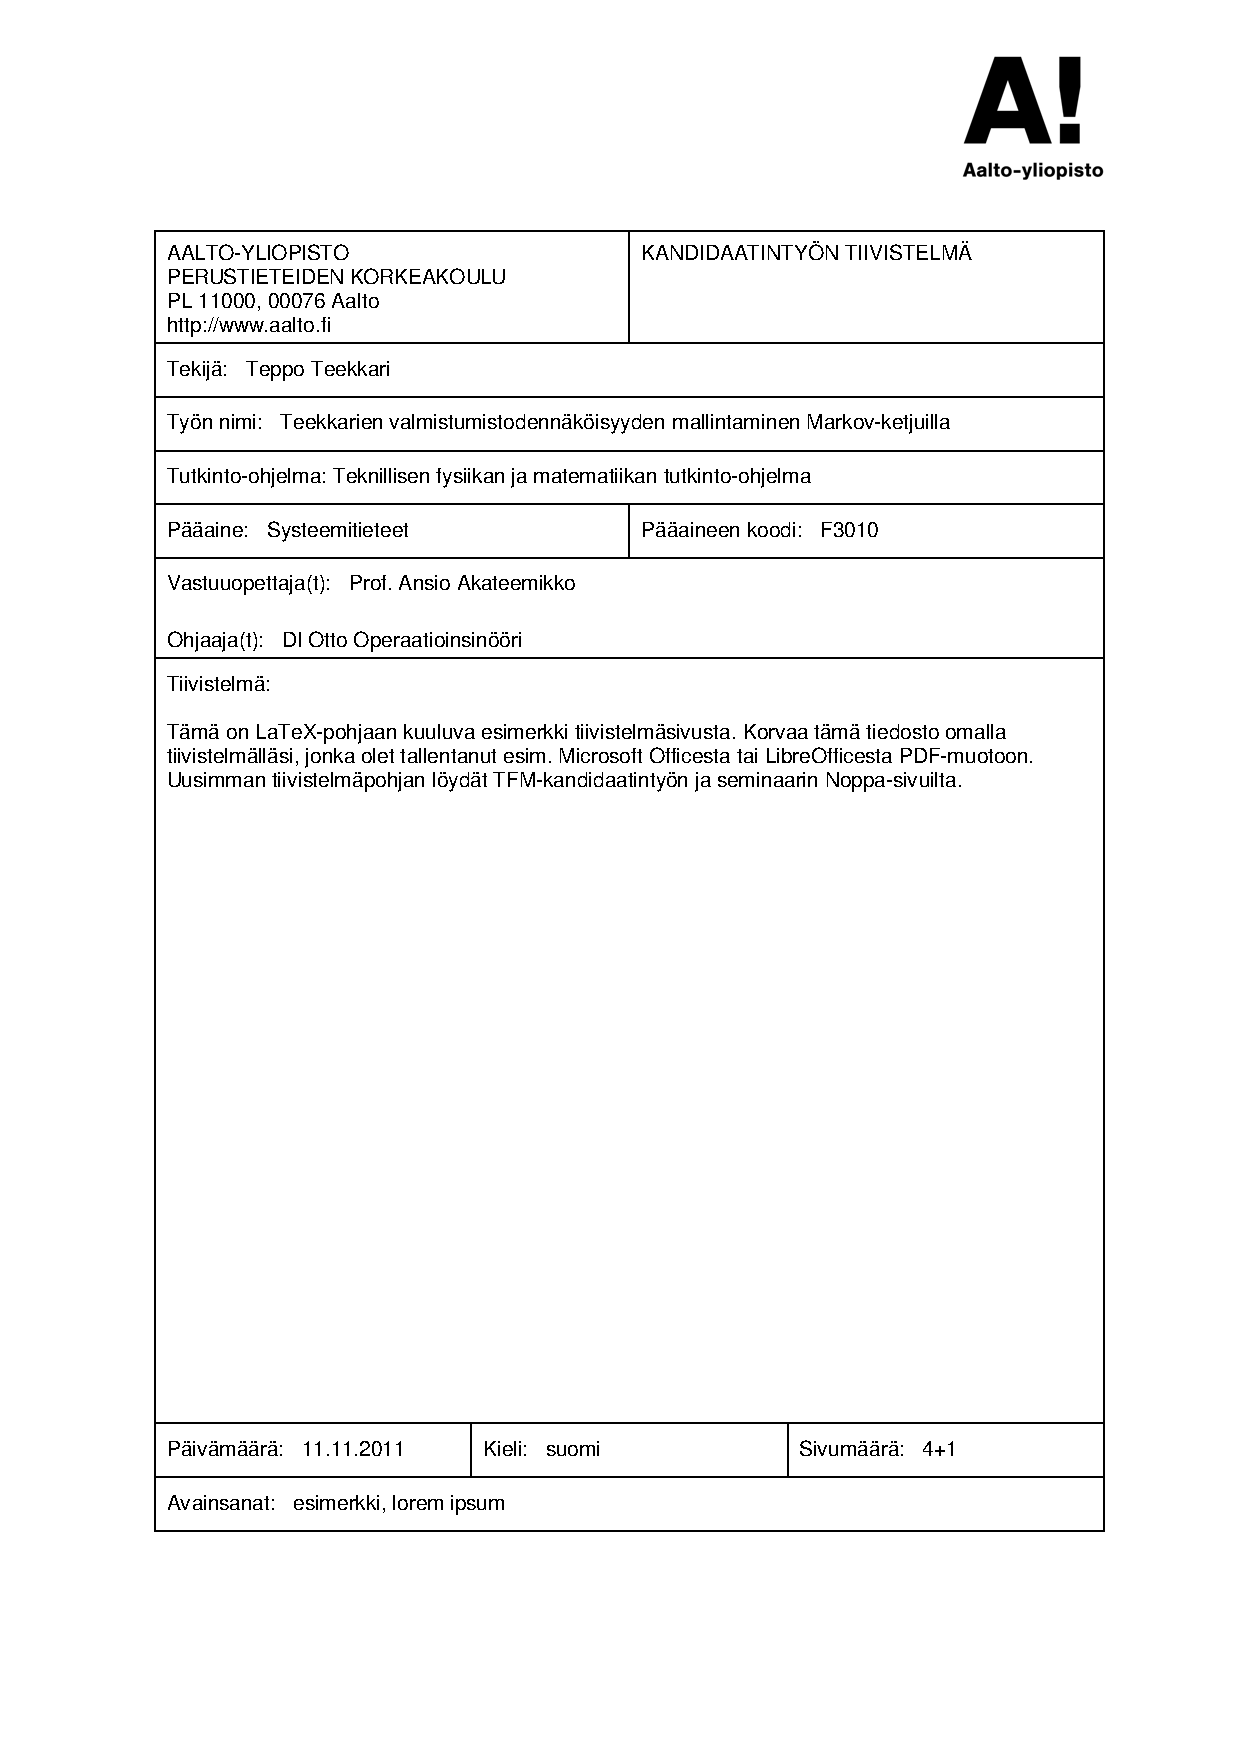
\includepdf{tiivistelma}

% Sisällysluettelo
\tableofcontents
\newpage

% Aloita todellinen sivunumerointi ensimmäisestä sisältösivusta
\pagestyle{fancy}

% Tyhjennetään kentät ja muotoilu
\fancyhf{}
\renewcommand{\headrulewidth}{0pt}
\renewcommand{\footrulewidth}{0pt}

% Sivunnumero ylhäällä oikealla
\rhead{\footnotesize \thepage} 
\pagenumbering{arabic}

% Ensimmäisellä sivulla ei kuitenkaan näytetä numeroa
\thispagestyle{empty} 


\section{Introduction}


There are a number of sources for real-life unconstrained nonlinear optimization problems from different fields of sciences and technologies. In general an unconstrained optimization problem can be formulated as
\begin{equation}
    \mathrm{min}_{\vect{x} \in \R^n} f(\vect{x}).
\end{equation}

Depending on the methods used, there may also be additional requirements for $f$, such as being continuously differentiable up to $n$ times or being convex i.e. having one unique global minimum. While there are a number of real-life problems that do satisfy these conditions they are often extremely complex. Therefore artificial problems are often used to develop and test optimization algorithms. \cite{test_function_collection_artifical}

The optimization algorithms are iterative processes that abuse the properties of the target function combined with the raw processing powers of computers. The commonly used methods are based on the same principle of having some termination condition checking if the minimum was found, and if not, continuing by choosing a direction and a step size and moving to the next point and repeating. The step size is often chosen by a separate algorithm called a line search, which transforms the target function into one-dimensional function of step size $\lambda$ and using the new function to calculate the optimal step size for each iteration of the main method. Similarly to the main methods, there are a number of different algorithms for finding the optimal step size, the simplest being just using a constant $\lambda$ for every iteration.

In this thesis we will be exploring the effects of line search method selection on the overall performance of the optimization method. Due to the limiting factor of the scope of the bachelor's thesis, this will be in no way a comprehensive statistical research. Instead the main goal is to provide insight on few use cases, primarily on the ones introduced on the Nonlinear Optimization (2018-2019) course in the Aalto University.

\todoinline{Should I mention the target functions, main methods and line search methods explored already here on intro?}

\todoinline{What is the recommended style for e.g. marking vectors?\\
Which equations should I numerate?}
    

\section{Theory}


\subsection{Target Functions}


\subsubsection{Choosing target functions}


One of the biggest factors effecting the performance of an optimization algorithm is the complexity of the target function we are using the method for. In this thesis we are going to focus on two different functions. Both of the functions are convex and differentiable since some of the methods we will be comparing require these properties. To increase the complexity of the problems a bit, we are going to use 50-dimensional versions of the two functions. Therefore we are going to pick functions that are defined in $\R^n$ or similar domain and then set $n = 50$.


\subsubsection{Step size function}


Each optimization method involves a step in form of $\mathrm{argmin}_{\lambda \in \mathbb{R}} {f(x_i + \lambda d_i})$. To programmatically produce this step, we are going to define step size function $g(\lambda)$ related to each of the target functions. Then on each iteration of the main optimization method, a new step size function is seeded with the updated point $\vect{x}$ and direction vector $\vect{d}$.


\subsubsection{Matrix Square Sum} \label{sect:matrix_square_sum}


The Matrix Square Sum is an extended version of the regular Sum Squares Function, which is defined as
\begin{equation}
    f(\mathbf{x})=f(x_1, ..., x_n)=\sum_{i=1}^{n}{ix_i^2}.
\end{equation}

To make Sum Squares problem less trivial, we are going modify it by adding three constants $A$, $b$ and $c$. Together they form what we are going to call a Matrix Square Sum function, defined as
\begin{equation}
    f(\vect{x}) = \norm{A \vect{x} + \vect{b}} ^ 2 + c \norm{\vect{x}} ^ 2,
\end{equation}

where $A$ is a positive definite (PD) $n \times n$ matrix, $\vect{x}$ and $\vect{b}$ are vectors of length $n$, and the scalar $c$ is a positive constant.

While $A$ could in theory be any $m \times n$ matrix, we are limiting it to a square PD-matrices only to ensure that the function is convex and has an unique global minimum. The matrix $A$ is formed in few steps by first generating an initial $n \times n$ matrix $A'$ with random values $a_{ij} \in [-0.5, 0.5]\ \forall\ i,j = 1 \dots n$. Then we attempt to make a PD-matrix by $A = 0.5 (A' + A'^\top)$. Finally, if  $A$ does not happen to be a PD-matrix yet, it is modified by the formula 
\begin{equation}
    A = A + (\abs{\lambda_{min}} + d) I,
\end{equation}
where $\lambda_{min}$ is the minimal eigenvalue of $A$ and $d$ is a constant. The value of $d$ also determines the A's condition number defined as $\frac{\lambda_{max}}{\lambda_{min}}$. Smaller values of $d$ make the function more elliptic and harder for gradient methods to solve, while larger values produce more circular gradient curves, which are easy for methods like Gradient Descent to solve. The value of $d$ used in the thesis is 5, resulting in condition number of around 6.5.

The values of $b$ and $c$ are also randomized so that for each element of $b$ applies $b_i \in [-0.5, 0.5]$ and $c$ is a scalar randomly generated from range $[-0.5, 0.5]$.

Some of the optimization methods require access to the function's gradient, Hessian matrix and the step size function with its first two derivatives, so let's calculate them in advance. While at it, we should also derive the formula for calculating the correct optima so we can use it to determine whether our algorithms produce the correct solution. Lets begin by expanding the function into more easily differentiable form:
\begin{align*}
    f(\vect{x}) &= \norm{A \vect{x} + \vect{b}} ^ 2 + c \norm{\vect{x}} ^ 2 \\
               &= (A \vect{x} + \vect{b})^\top(A \vect{x} + \vect{b}) + c \trans{x} \vect{x} \\
               &= (\trans{x} A^\top + \trans{b})(A\vect{x} + \vect{b}) + c \trans{x} \vect{x} \\
               &= \trans{x} A^\top A \vect{x} + \vect{x} A^\top \vect{b} + \trans{b} A \vect{x} + \trans{b} \vect{b} + c \trans{x} \vect{x} \\
               &= \trans{x} A^\top A \vect{x} + 2 \trans{b} A \vect{x} + \trans{b} \vect{b} + c \trans{x} \vect{x}.
\end{align*}

Now let's calculate the gradient and then Hessian matrix:
\begin{align}
    \nabla f(\vect{x}) &= \nabla(\trans{x} A^\top A \vect{x}) + 2 \nabla(\trans{b} A \vect{x}) + \nabla(\trans{b} \vect{b}) + \nabla(c \trans{x} \vect{x}) \nonumber \\
    &= (\trans{x} A^\top A)^\top + A^\top A \vect{x} + 2 (\trans{b} A)^\top + c (\trans{x})^\top + c \vect{x} \nonumber \\
    &= 2 A^\top A \vect{x} + 2 A^\top \vect{b} + 2 c \vect{x} \\
    &\nonumber \\
    \textbf{H} &= \nabla^2 f(\vect{x}) = 2 A^\top A + 2 c I
\end{align}

From the gradient we get the necessary optimality condition
\begin{equation}
    (A^\top A + c I) \vect{x} = - A^\top \vect{b}
\end{equation}
and because the function is convex (the Hessian is positive definite for all $\vect{x} \in \mathbb{R}^n$), we get the unique optimal solution
\begin{equation}
    \vect{x} = - (A^\top A + c I)^{-1} A^\top \vect{b}
\end{equation}

Let's now form the step size function and its derivatives:
\begin{align}
    g(\lambda) =\ &f(\vect{x} + \lambda \vect{d}) = \norm{A (\vect{x} + \lambda \vect{d}) + \vect{b}} ^ 2 + c \norm{(\vect{x} + \lambda \vect{d})} ^ 2 \nonumber \\
    =\ &\lambda \trans{d} A^\top ( 2 A \vect{x} + \lambda A \vect{d} + 2 \vect{b}) + \trans{x} A^\top ( A \vect{x} + 2 \vect{b} ) + \trans{b} \vect{b} \\
    &+ c ( \trans{x} \vect{x} + 2 \lambda \trans{d} \vect{x} + \lambda ^ 2 \trans{d} \vect{d}) \nonumber \\
    g'(\lambda) =\ &\trans{d} A^\top ( 2 A \vect{x} + 2 \lambda A \vect{d} + 2 \vect{b} ) + 2 c \trans{d} ( \vect{x} + \lambda \vect{d} ) \\
    g''(\lambda) =\ &2 \trans{d} ( A^\top A \vect{d} + c \vect{d})
\end{align}


\subsubsection{Negative Entropy}


The second target function reviewed is a variation of entropy maximization problem, in which the maximation problem is inverted therefore making it a minimization problem. We will be calling this convex minimization problem a Negative Entropy problem and it can be formulated as follows:
\begin{equation}
	f(\vect{x}) = \sum_{i=1}^{n} x_i \log x_i,
\end{equation}
where $\vect{x} \in \mathbb{R}_{> 0}^n$. Since the domain is now limited we have to do some adjustments to our algorithms, which we will get into in a moment.

The global minima of the function can be found by calculating the zero point of the gradient:
\begin{align}
    \nabla f(\vect{x}) &= \frac{\delta}{\delta x_i} \sum_{i=1}^{n} x_i \log x_i \\
                      &= \sum_{i=1}^{n} (\log x_i + 1) = 0.
\end{align}

Because the $\log x_i + 1$ is truly positive, the answer is the same for every term $x_i$. Therefore we get the minima: $\log x_i = -1 \Leftrightarrow x_i = \frac{1}{e}$, for every $i = 1 \dots n$.

In addition to the gradient, we need to calculate the Hessian matrix and the one dimensional step size function $g(\lambda) = f(\vect{x} + \lambda \vect{d})$ with its first and second derivatives in regard to $\lambda$.

As we already know the gradient of $f$, the Hessian can be derived with ease since $\frac{\delta^2}{\delta x_i \delta x_j} \sum_{i=1}^{n} x_i \log x_i = 0$ for every $i, j$ where $i \neq j$. For the diagonal cases, i.e. when $i = j$, we are left with the second derivative $\frac{1}{x_i}$. Therefore we get the following Hessian matrix:
\begin{equation}
    \textbf{H} =
    \begin{bmatrix}
    x_1^{-1} & 0        & 0      & \dots  & 0      \\
    0        & x_2^{-1} & 0      & \dots  & 0      \\
    \vdots   & \vdots   & \vdots & \ddots & \vdots \\
    0        & 0        & 0      & \dots  & x_n^{-1}
\end{bmatrix}.
\end{equation}

Finally, the step size function for $\lambda$ with its first two derivatives are as follows:
\begin{align}
    g(\lambda) &= \sum_{i=1}^{n} (x_i + \lambda d_i) \log (x_i + \lambda d_i) \\
    g'(\lambda) &= \sum_{i=1}^{n} d_i (\log(x_i + \lambda d_i) + 1) \\
    g''(\lambda) &= \sum_{i=1}^{n} \frac{d_i^2}{x_i + \lambda d_i}.
\end{align}

Because the domain of this function is only positive numbers, we are going to have make some changes to our starting points, parameters and algorithms. Therefore the starting point must only have positive coordinates and the following domain limiter was added to the line search algorithms which update the starting point so that it could otherwise go negative:

\begin{algorithm}[H]
\caption{Domain Limiter}
\label{alg_domain_limiter}
\begin{algorithmic}[1]
\STATE \textbf{initialize} $\gamma \in [0, 1]$
\WHILE{min $(\vect{x} + \lambda \vect{d}) <= 0$}
    \STATE $\lambda = \lambda \gamma$
\ENDWHILE
\RETURN $\lambda$
\end{algorithmic}
\end{algorithm}

The domain limiter will be called from all of the line search methods before any evaluation of $f(\lambda)$ to reduce the step size to such value that it prevents evaulation of negative logarithms. In the context of this thesis we are going to set $d = 0.99$, but it could also be added as a parameter for each of the line search functions as some methods will require more iterations on the while-loop than others.


\subsection{Main Methods}


The main methods as I call them in the scope of this thesis are methods for finding minimums for unconstrained, differentiable and convex functions. While some of the methods or line search methods do not require all these properties, they are included anyway for this analysis.


\subsubsection{Newton's Method}


Newton's method is \todo{source?} commonly used for finding global minimums for differentiable and convex functions. The algorithm is a more general version of its line search version, utilizing the gradient and hessian matrix of the function instead of its first and second single derivatives.

\begin{algorithm}[H]
\caption{Newton's Method}
\label{alg_newtons}
\begin{algorithmic}[1]
\STATE \textbf{initialize} $l > 0, k = 0$, $k_{max} \in \N$, $\vect{x} = \vect{x_0} \in \R^n$, step size function $g_{\vect{x}, \vect{d}}(\lambda)$ and line search method $L$.
\WHILE{$\norm{\nabla \theta(\vect{x})} > l$ \AND $k < k_{max}$}
    \STATE $\vect{d} = -H(\vect{x})^{-1} \nabla \theta(\vect{x})$
    \STATE $\lambda = L(g_{\vect{x}, \vect{d}})$
    \STATE $\vect{x} = \vect{x} + \lambda \vect{d}$
    \STATE $k = k + 1$
\ENDWHILE
\RETURN $\lambda$
\end{algorithmic}
\end{algorithm}


\subsubsection{Gradient Descent Method}


Gradient descent method can be interpret as a simpler version of Newton's method as it only advances one gradient at a time. The algorithm is exactly the same as in Newton's method except for line 3 where the descent direction $d$ is calculated in a little bit simpler manner.

\begin{algorithm}[H]
\caption{Gradient Descent Method}
\label{alg_gradient_descent}
\begin{algorithmic}[1]
\STATE \textbf{initialize} $l > 0, k = 0$, $k_{max} \in \N$, $\vect{x} = \vect{x_0} \in \R^n$, step size function $g_{\vect{x}, \vect{d}}(\lambda)$ and line search method $L$.
\WHILE{$\norm{\nabla \theta(\vect{x})} > l$ \AND $k < k_{max}$}
    \STATE $\vect{d} = -\nabla \theta(\vect{x})$
    \STATE $\lambda = L(g_{\vect{x}, \vect{d}})$
    \STATE $\vect{x} = \vect{x} + \lambda \vect{d}$
    \STATE $k = k + 1$
\ENDWHILE
\RETURN $\lambda$
\end{algorithmic}
\end{algorithm}


\subsubsection{Conjugate Gradient Method}


Conjugate gradient method uses the information from the previous and current iterations to calculate ratio of gradients to calculate optimal next point. The method should theoretically \todo{source?} require less steps than gradient descent method.

The algorithm involves a second loop which runs for $n$ times per every iteration on the main loop. The $n$ is equal to the dimensions of the problem (i.e. $\mathrm{dim}(\vect{x})$) and also the inner iterations are calculated towards the total iterations.

\begin{algorithm}[H]
\caption{Conjugate Gradient Method}
\label{alg_conjugate_gradient}
\begin{algorithmic}[1]
\STATE \textbf{initialize} $l > 0, k = 0$, $k_{max} \in \N$, $\alpha \in \R$, $\vect{x} = \vect{x_0} \in \R^n$, step size function $g_{\vect{x}, \vect{d}}(\lambda)$ and line search method $L$.
\STATE $\vect{d} = -\nabla \theta(\vect{x})$
\WHILE{$\norm{\nabla \theta(\vect{x})} > l$ \AND $k < k_{max}$}
    \STATE $\vect{y} = \vect{x}$
    \FOR{$i = 1 \dots n$}
        \STATE $\lambda = L(g_{\vect{y}, \vect{d}})$
        \STATE $\vect{y_{prev}} = \vect{y}$, \ $\vect{y} = \vect{y} + \lambda \vect{d}$
        \STATE $\alpha = \frac{\nabla \theta(\vect{y})^2}{\nabla \theta(\vect{y_{prev}})^2}$
        \STATE $\vect{d} = -\nabla \theta(\vect{y}) + \alpha \vect{d}$
        \STATE $k = k + 1$
    \ENDFOR
    \STATE $\vect{x} = \vect{y}$, \ $\vect{d} = \nabla \theta(\vect{x})$
\ENDWHILE
\RETURN $\lambda$
\end{algorithmic}
\end{algorithm}


\subsubsection{Heavy Ball Method}


Heavy ball method is basically an extension of gradient descent as only adds one term for the direction vector calculation step. The name of the method comes from the \todo{source?} physical representation of momentum of a ball rolling downhill. The algorithm for the method is basically the same as Gradient descent with a single additional term with multiplier $\beta$ in descent direction $d$.

\begin{algorithm}[H]
\caption{Heavy Ball Method}
\label{alg_heavy_ball}
\begin{algorithmic}[1]
\STATE \textbf{initialize} $l > 0, k = 0$, $k_{max} \in \N$, $\beta \in \R$, $\vect{x} = \vect{x_{prev}} = \vect{x_0} \in \R^n$, step size function $g_{\vect{x}, \vect{d}}(\lambda)$ and line search method $L$.
\WHILE{$\norm{\nabla \theta(\vect{x})} > l$ \AND $k < k_{max}$}
    \STATE $\vect{d} = -\nabla \theta(\vect{x}) + \beta (\vect{x} - \vect{x_{prev}})$
    \STATE $\lambda = L(g_{\vect{x}, \vect{d}})$
    \STATE $\vect{x_{prev}} = \vect{x}$, \ $\vect{x} = \vect{x} + \lambda \vect{d}$
    \STATE $k = k + 1$
\ENDWHILE
\RETURN $\lambda$
\end{algorithmic}
\end{algorithm}


\subsection{Line Search Methods}


Most line search methods are based on a single idea, which we are going to call the theorem 1:

Theorem 1: Let $\theta$ : R $\rightarrow$ R be strictly quasiconvex over the interval $[a, b]$, and let $\lambda$, $\mu$ $\in$ $[a, b]$ such that $\lambda < \mu$. If $\theta(\lambda) > \theta(\mu)$, then $\theta(z) \geq \theta(\mu)$
for all $z \in [a, \lambda]$. If $\theta(\lambda) \leq \theta(\mu)$, then $\theta(z) \leq \theta(\lambda)$ for all $z \in [\mu, b]$. \cite{course_material_nonlinear_optimisation}


\subsubsection{Constant Step Size}


While not actually a search, the use of single step size value $\lambda$ is sometimes enough to provide correct and high performance solutions for the main methods. In this thesis I will be considering constant $\lambda$ as one of the search methods to provide comprehensive comparison.

\begin{center}
\rowcolors{2}{white}{gray!5}
\captionof{table}{Parameters tested for ConstantSearch}
\label{tab:params_ConstantSearch}
\begin{tabular}{|c|c|c|}
\hline
\rowcolor{gray!25}
Parameter & MatrixSquareSum & NegativeEntropy \\
\hline
$\lambda$ & 0.0001, 0.1, 0.25, 0.5, 0.9 & 0.1, 0.25, 0.5 \\
\hline
\end{tabular}
\end{center}


\subsubsection{Golden Section Search}

While golden section and fibonacci numbers are closely related, the golden section search does take much more straight forward way for calculating the new step size bounds using the approximation of $\phi = 0.618$. \todoinline{is this approx good enough or should I add more digits?}

\begin{algorithm}[H]
\caption{Golden Section Search}
\label{alg_golden_section}
\begin{algorithmic}[1]
\STATE \textbf{initialize} tolerance $l > 0$, $\alpha = 0.618$, $k = 0$, $k_{max} \in \N$, $(a, b) \in \R$.
\STATE $\lambda = a + (1 - \alpha) (b - a)$, $\mu = a + \alpha (b - a)$.
\WHILE{$b - a > l$ \AND $k < k_{max}$}
    \IF{$\theta(\lambda) > \theta(\mu)$}
        \STATE $a = \lambda$, \ $\lambda = \mu$, \ $\mu = a + \alpha (b - a)$
    \ELSE
        \STATE $b = \mu$, \ $\mu = \lambda$, \ $\lambda = a + (1 - \alpha) (b - a)$
    \ENDIF
    \STATE $k = k + 1$
\ENDWHILE
\RETURN $\lambda = \frac{a + b}{2}$
\end{algorithmic}
\end{algorithm}

\begin{center}
\rowcolors{2}{white}{gray!5}
\captionof{table}{Parameters tested for GoldenSectionSearch}
\label{tab:params_GoldenSectionSearch}
\begin{tabular}{|c|c|c|}
\hline
\rowcolor{gray!25}
Parameter & MatrixSquareSum & NegativeEntropy \\
\hline
$a$ & -10, -5 & -10, -5 \\
$b$ & 10, 5 & 10, 5 \\
$l$ & 0.0001, 1e-07 & 0.0001, 1e-07 \\
\hline
\end{tabular}
\end{center}


\subsubsection{Bisection Search}


Bisection method is \todo{source?} commonly used line search method for differentiable functions. It basically narrows down the optimal step size range using the first derivative of the target function as a direction of which bound to move next.

\begin{algorithm}[H]
\caption{Bisection Search}
\label{alg_bisection}
\begin{algorithmic}[1]
\STATE \textbf{initialize} $l > 0, k = 0$, $k_{max} \in \N$, $(a, b) \in \R$.
\WHILE{$\abs{b - a} > l$ \AND $k < k_{max}$}
    \STATE $\lambda = \frac{b + a}{2}$
    \IF{$\theta'(\lambda) = 0$}
        \RETURN $\lambda$
    \ELSIF{$\theta'(\lambda) > 0$}
        \STATE $b = \lambda$
    \ELSE
        \STATE $a = \lambda$
    \ENDIF
    \STATE $k = k + 1$
\ENDWHILE
\RETURN $\lambda = \frac{a + b}{2}$
\end{algorithmic}
\end{algorithm}

\begin{center}
\rowcolors{2}{white}{gray!5}
\captionof{table}{Parameters tested for BisectionSearch}
\label{tab:params_BisectionSearch}
\begin{tabular}{|c|c|c|}
\hline
\rowcolor{gray!25}
Parameter & MatrixSquareSum & NegativeEntropy \\
\hline
$a$ & -10, -5 & -10, -5 \\
$b$ & 10, 5 & 10, 5 \\
$l$ & 0.0001, 1e-07 & 0.0001, 1e-07 \\
\hline
\end{tabular}
\end{center}


\subsubsection{Dichotomous Search}


Dichotomous search is an example of sequentical searches. It uses the information of the previous evaulation of $\theta$ resulting in higher performance than e.g. uniform search.

\begin{algorithm}[H]
\caption{Dichotomous Search}
\label{alg_dichotomous}
\begin{algorithmic}[1]
\STATE \textbf{initialize} $l > 0, k = 0$, $k_{max} \in \N$, $(a, b) \in \R$.
\WHILE{$b - a > l$ \AND $k < k_{max}$}
    \STATE $\lambda = \frac{b + a}{2} - \epsilon$, \ $\mu = \frac{b + a}{2} + \epsilon$
    \IF{$\theta(\lambda) < \theta(\mu)$}
        \STATE $b = \mu$
    \ELSE
        \STATE $a = \lambda$
    \ENDIF
    \STATE $k = k + 1$
\ENDWHILE
\RETURN $\lambda = \frac{a + b}{2}$
\end{algorithmic}
\end{algorithm}

\begin{center}
\rowcolors{2}{white}{gray!5}
\captionof{table}{Parameters tested for DichotomousSearch}
\label{tab:params_DichotomousSearch}
\begin{tabular}{|c|c|c|}
\hline
\rowcolor{gray!25}
Parameter & MatrixSquareSum & NegativeEntropy \\
\hline
$a$ & -10, -5 & -10, -5 \\
$b$ & 10, 5 & 5, 10 \\
$\epsilon$ & 1e-07, 1e-08 & 1e-06, 1e-07 \\
$l$ & 0.0001 & 0.0001, 1e-05 \\
\hline
\end{tabular}
\end{center}



\subsubsection{Fibonacci Search}


Fibonacci is an interesting \todo[color=green!40]{or what term to use for methods that do not use derivative?} numerical method for providing optimal step sizes using fibonacci numbers when calculating the bounds for the step size. [better explanation of why this works?] The calculation may be somewhat heavy due to the requirement of calculating $n$ fibonacci numbers, where $n$ is determined by the required accuracy i.e. tolerance. However, in some real life applications these fibonacci numbers may of course be precalculated. In this thesis I will not be using a table for the fibonacci values but instead actually calculate them using a while loop. The iteration count for finding the fibonacci numbers will not be included in the performance comparison, but the time taken to find the values is included. \todoinline{is this fine, or should I also report the fibonacci iteration count and time?}

\begin{algorithm}[H]
\caption{Fibonacci Search}
\label{alg_fibonacci}
\begin{algorithmic}[1]
\STATE \textbf{initialize} $l > 0, \epsilon > 0, k = 0$, $k_{max} \in \N$, $(a, b) \in \R, n = \mathrm{min}_n \{ \frac{b - a}{F_n} \leq l \}$.
\STATE $\lambda = a + \frac{F_{n-2}}{F_n} (b - a)$, \  $\mu = a + \frac{F_{n-1}}{F_n} (b - a)$
\WHILE{$k \leq n - 1$ \AND $k < k_{max}$}
    \IF{$\theta(\lambda) < \theta(\mu)$}
        \STATE $a = \lambda$, \ $\lambda = \mu$, $\mu = a + \frac{F_{n-k-1}}{F_{n-k}} (b - a)$
    \ELSE
        \STATE $b = \mu$, \ $\lambda = \mu$, $\lambda = a + \frac{F_{n-k-2}}{F_{n-k}} (b - a)$
    \ENDIF
    \STATE $k = k + 1$
\ENDWHILE
\STATE $\lambda = \theta(\lambda)$
\IF{$\theta(\lambda) > \theta(\mu + \epsilon)$}
    \STATE $a = \lambda$
\ELSE
    \STATE $b = \mu$
\ENDIF
\RETURN $\lambda = \frac{a + b}{2}$
\end{algorithmic}
\end{algorithm}

The $F_n$ represents $n$:th Fibonacci number. To optimize algorithm performance, the values of $F_n$ could be pre-evaluated but for our use case we are just going to generate the Fibonacci numbers using single loop algorithm of time complexity $O(n)$.

\begin{center}
\rowcolors{2}{white}{gray!5}
\captionof{table}{Parameters tested for FibonacciSearch}
\label{tab:params_FibonacciSearch}
\begin{tabular}{|c|c|c|}
\hline
\rowcolor{gray!25}
Parameter & MatrixSquareSum & NegativeEntropy \\
\hline
$a$ & -10, -5 & -10, -5 \\
$b$ & 10, 5 & 10, 5 \\
$\epsilon$ & 0.01, 1e-05, 1e-08 & 0.01, 1e-05, 1e-08 \\
$l$ & 0.0001, 1e-07 & 0.0001, 1e-07 \\
\hline
\end{tabular}
\end{center}


\subsubsection{Uniform Search}


Uniform search works by dividing a constrained section of a function into intervals, then choosing the interval with the lowest value and performing the same procedure again for it. To increase the precision of the method we also increase the number of intervals we divide the newly selected interval into.

More formally: break $[a, b]$ into $n$ uniform intervals of size $\delta$, which leads to $n + 1$ grid points $a_0 + k \delta$ with $b = a_n = a_0 + n\delta,\ k = 0, . . . , n$. \cite{course_material_nonlinear_optimisation}

In addition we are going to define $n$ as the interval count and $m$ as the interval count multiplier.

\begin{algorithm}[H]
\caption{Uniform Search}
\label{alg_uniform}
\begin{algorithmic}[1]
\STATE \textbf{initialize} $l > 0, k = 0$, $(k_{max}, n) \in \N$, $(a, b, m) \in \R$
\STATE $s = \frac{b - a}{n}$, \ $p_{min} = a$
\WHILE{$s > l$ \AND $k < k_{max}$}
    \FOR{$i = 0, \dots, n$}
        \STATE $x = a + i s$
        \IF{$\theta(x) < \theta(p_{min})$}
            \STATE $p_{min} = x$
        \ENDIF
        \STATE $k = k + 1$
    \ENDFOR
    \STATE $a = p_{min} - s$, \ $b = p_{min} + s$
    \STATE $n = \floor{n m}$, \ $s = \frac{b - a}{n}$
\ENDWHILE
\RETURN $\lambda = \frac{a + b}{2}$
\end{algorithmic}
\end{algorithm}

\begin{center}
\rowcolors{2}{white}{gray!5}
\captionof{table}{Parameters tested for UniformSearch}
\label{tab:params_UniformSearch}
\begin{tabular}{|c|c|c|}
\hline
\rowcolor{gray!25}
Parameter & MatrixSquareSum & NegativeEntropy \\
\hline
$a$ & -10, -5 & -10, -5 \\
$b$ & 10, 5 & 10, 5 \\
$n$ & 10, 100 & 10, 100 \\
$m$ & 1, 1.5 & 1, 1.5 \\
$l$ & 0.0001, 1e-07 & 0.0001, 1e-07 \\
\hline
\end{tabular}
\end{center}


\subsubsection{Newton's Search}


Newton's method is another very common example of line search methods. Similarily to bisection method, Newton's method requires the target function to be differentiable up to two times as it uses the ratio of first and second derivatives to move the optimal step size forward.

\begin{algorithm}[H]
\caption{Newton's Search}
\label{alg_newtons_search}
\begin{algorithmic}[1]
\STATE \textbf{initialize} $l > 0, k = 0$, $k_{max} \in \N$, $\lambda \in \R$
\WHILE{$\abs{\theta'(\lambda)} > l$ \AND $k < k_{max}$}
    \STATE $\lambda = \lambda -\frac{\theta'(\lambda)}{\theta''(\lambda)}$
    \STATE $k = k + 1$
\ENDWHILE
\RETURN $\lambda$
\end{algorithmic}
\end{algorithm}

\begin{center}
\rowcolors{2}{white}{gray!5}
\captionof{table}{Parameters tested for NewtonsSearch}
\label{tab:params_NewtonsSearch}
\begin{tabular}{|c|c|c|}
\hline
\rowcolor{gray!25}
Parameter & MatrixSquareSum & NegativeEntropy \\
\hline
$\lambda$ & 1, 5, 10, 50 & 0.5, 1.0 \\
$l$ & 1e-07, 1e-08 & 1e-06, 1e-07 \\
\hline
\end{tabular}
\end{center}

\subsubsection{Armijo's Search}

Armijo's search is the only backtracking method of the ones included in this thesis. \todo[inline]{include more in depth explanation of backtracking algorithms?}

\begin{algorithm}[H]
\caption{Armijo's Search}
\label{alg_armijo}
\begin{algorithmic}[1]
\STATE \textbf{initialize} $l > 0, k = 0$, $k_{max} \in \N$, $(\lambda, \alpha, \beta) \in \R$
\STATE $\theta_0 = \theta(0)$, \ $\theta'_0 = \theta'(0)$
\WHILE{$\theta(\lambda) > \theta_0 + \alpha \lambda \theta'_0$ \AND $k < k_{max}$}
    \STATE $\lambda = \lambda \beta$
    \STATE $k = k + 1$
\ENDWHILE
\RETURN $\lambda$
\end{algorithmic}
\end{algorithm}


\section{Methods}


Our goal is to determine how does the selection of line search method effect the overall performance of an optimization method. To answer this question with the resources introduced in the theory section, we first need to tackle the problem of choosing parameters.


\subsection{Parameter Selection}

Optimization method parameter selection is a whole large topic of its own, and it is not our main focus on this thesis. Therefore a very straightforward method for picking the parameters is going to be appropriate.

Using the same setup as when we are comparing the performances of different method combinations, we can also compare the effects of different parameters. Using the manually picked parameter values shown in the theory section, we can programmatically generate all the permutations for each parameter and optimization method combination.

\subsection{Starting Point Selection}

So we are going to compare the performances of each line search method and main method combination with their related parameter options. We are running the tests with 100 starting points of dimension $n = 50$. For practical reasons we are also going to use a limited space for the points to be randomized from.

Let a single starting point be $x = \{x_1, x_2, \dots x_{50}\}$. For MatrixSquareSum the points are generated so that for each point applies $x_i \in  [-10, 10]\ \forall\ i$. Because NegativeEntropy's domain is $\R_{>0}$, the same rule applies but with the bounds being $]0, 10]$ instead.

Since we are interested in overall performance, we prefer starting points that are random but evenly distributed so that no two point are the same, or too close to each other. To generate a point distribution which is random but evenly filled with points, we use the following algorithm.

\begin{algorithm}[H]
\caption{Generating Even Distribution of Random Starting Points}
\label{alg_x0_distribution}
\begin{algorithmic}[1]
\STATE \textbf{initialize} $(d_{min}, x_{min}, x_{max}) \in \R, (n, p) \in \N, \vect{x}_1 = \mathbf{random}_{n}(x_{min}, x_{max})$, $q = 1$
\WHILE{$i < p$}
    \STATE $\vect{y} = \mathbf{random}_{n}(x_{min}, x_{max})$
    \STATE $\mathrm{ok} =$ \TRUE
    \FOR{$j = 1 \dots q$}
        \IF{$\norm{\vect{x}_j - \vect{y}} < d_{min}$}
            \STATE $\mathrm{ok} = $ \FALSE
            \STATE \textbf{break}
        \ENDIF
    \ENDFOR
    \IF{ok}
        \STATE $q = q + 1$, \ $i = i + 1$
        \STATE $\vect{x}_q = \vect{y}$
    \ENDIF
\ENDWHILE
\RETURN $\{ x_1, x_2, ..., x_p\}$
\end{algorithmic}
\end{algorithm}

The algorithm generates $p$ points of dimension $n$. The generated points are stored in variables $x_i$. The function $\mathbf{random}_n(x_{min}, x_{max})$ generates a single point of dimension $n$ filled with random values from the range $[x_{min}, x_{max}]$. On every iteration, we test to see if the newly generated point is closer than $d_{min}$ to some existing point and if so, we discard the new point and try again.

This is by means not a perfect algorithm since its performance heavily depends on the $d_{min}$ value used. The minimum distance selection depends on the point count and the available point space: too high values cause the algorithm to end up on infinite loop and too low values do not provide the even distribution we are looking for. Via trial and error the values presented in table \ref{tab:dmin_values} are picked.

\begin{table}[H]
\centering
\captionof{table}{The minimum Eucleidean distances used for different target functions on distributions of 100 and 1000 points.}
\label{tab:dmin_values}
\begin{tabular}{|r|r|r|}
\hline
\rowcolor[HTML]{C0C0C0} 
Point count                       & MSS $d_{min}$ & NE $d_{min}$ \\ \hline
\cellcolor[HTML]{EFEFEF}100  & 56           & 28          \\ \hline
\cellcolor[HTML]{EFEFEF}1000 & 48           & 24          \\ \hline
\end{tabular}
\end{table}

After successfully generating the starting points once, we are going to save them into a file from which they are loaded during future runs. This way we maintain the same level of randomness for each run.

\subsection{Randomizing Target Function}

In addition to randomizing the starting points, we are going to use randomized parameters for Matrix Square Sum target function. The values of parameters $A$, $b$ and $c$ are going to be randomized as described in section \ref{sect:matrix_square_sum} but for each starting point separately. To control the randomness between runs, we give the function a random seed of the index of the current point. This way we end up with number of random functions equal to the number of starting points used. Combined with the saving of points, we can guarantee to get the same setup for each run.

\subsection{Comparing Performance}


There are multiple metrics that we could analyze, like algorithm success rate, main method or line search duration, iterations or function calls. The most important metric we are going to focus on is the success rate i.e. from how many of the 1000 starting points did the algorithm reach correct optimum. The solution is interpret as correct if the first 8 decimals of the found solution and correct one match.
Since it is excepted that most of the algorithms find the solution correctly every time, we also need a secondary comparison metric. Here we choose to use the total duration of the algorithm, since it is often the most interesting value for real life use cases and it is comparable within different methods unlike for example total iteration count. The other metrics will also be recorded and listed in the results section, but they will not be taken into consideration when scoring the methods.

% Performance comparison is going to be based mostly on total iterations meaning iterations of main method plus total iterations of the line search methods that the main method ran. The iterations of main method and line search methods are treated as equally valuable. Execution times are also recorded but not used as primary tool for performance tracking since with such little repetitions and the value of $n$ certain randomness plays too big of a part in the duration parameter. In addition, duration is heavily dependant on the programming language and style used so while the results could be comparable within the same language, they might behave differently under another setup. In comparison iterations are somewhat universal and thus make a better measure for performance. Another aspect that is recorded is the total number of function calls $n_f$ performed by both the main method and line search together. All the calls of $\theta$, its gradient and Hessian matrix, as well as the function calls of the step size function $f(\vect{x} + \lambda \vect{d})$ and its derivatives made by the line search method are calculated towards the same total count. This number is used as a secondary tool for comparison of the algorithms' performance.


\subsubsection{Parameter Selection}


\section{Results}

The results are going to be represented in a table with average performances of each line search method for each permutation of main methods and target functions. The performances are calculated using the best parameters found for each setup as described in the previous section. The algorithms are run with a similar setup as when calculating the best parameters, but this time with 1000 evenly randomized starting points instead of 100. Again for each starting point a unique target function configuration is generated in the case of MatrixSquareSum using the same randomizing rules as described in the previous section. The random seeds were again starting point indices i.e. integers from 0 to 1000.

After running the performance tests, we are left with the results introduced in the following eight tables. The row's of the table show the line search method used, the success rate of the algorithm, average duration, iteration count and function calls of the algorithm. The function call count includes all calls to the function and to its gradients or step size functions. In addition to these, the average duration and iterations taken by the line search algorithm alone is listed in the result tables. A table including all eight line search methods with their representative performances is generated for each main method and target function combination.


\begin{center}
\rowcolors{2}{white}{gray!5}
\captionof{table}{Average performances of NewtonsMethod when minimizing MatrixSquareSum using different line search methods and 1000 randomly generated starting points}
\label{tab:performance_results_MSS_NM}
\begin{tabular}{|l|r|r|r|r|r|r|}
\hline
\rowcolor{gray!25}
\multicolumn{1}{|c|}{Line Search Name} & \multicolumn{1}{c|}{$s$ (\%)} & \multicolumn{1}{c|}{$t$ (ms)} & \multicolumn{1}{c|}{$k$} & \multicolumn{1}{c|}{$f_n$} & \multicolumn{1}{c|}{$t_{LS}$ (ms)} & \multicolumn{1}{c|}{$k_{LS}$} \\
ConstantSearch & 100.0 & 445.8 & 1.0 & 7.0 & 0.0 & 0.0 \\
GoldenSectionSearch & 100.0 & 445.0 & 1.0 & 101.0 & 2.6 & 47.0 \\
BisectionSearch & 99.6 & 535.9 & 1.0 & 35.0 & 89.0 & 28.0 \\
DichotomousSearch & 100.0 & 429.1 & 1.0 & 77.0 & 3.3 & 35.0 \\
FibonacciSearch & 100.0 & 453.2 & 1.0 & 119.0 & 4.5 & 55.0 \\
UniformSearch & 100.0 & 455.0 & 1.0 & 156.0 & 7.2 & 148.0 \\
NewtonsSearch & 100.0 & 443.5 & 1.0 & 8.0 & 0.5 & 0.0 \\
ArmijoSearch & 100.0 & 424.2 & 1.0 & 10.0 & 0.9 & 0.0 \\
\hline
\end{tabular}
\end{center}

\begin{center}
\rowcolors{2}{white}{gray!5}
\captionof{table}{Average performances of GradientDescentMethod when minimizing MatrixSquareSum using different line search methods and 1000 randomly generated starting points}
\label{tab:performance_results_MSS_GDM}
\begin{tabular}{|l|r|r|r|r|r|r|}
\hline
\rowcolor{gray!25}
\multicolumn{1}{|c|}{Line Search Name} & \multicolumn{1}{c|}{$s$ (\%)} & \multicolumn{1}{c|}{$t$ (ms)} & \multicolumn{1}{c|}{$k$} & \multicolumn{1}{c|}{$f_n$} & \multicolumn{1}{c|}{$t_{LS}$ (ms)} & \multicolumn{1}{c|}{$k_{LS}$} \\
ConstantSearch & 98.9 & 4681.2 & 2942.0 & 8828.9 & 141.2 & 0.0 \\
GoldenSectionSearch & 99.4 & 283.7 & 33.1 & 1784.1 & 155.4 & 841.0 \\
BisectionSearch & 99.4 & 823.5 & 33.0 & 696.6 & 749.8 & 594.5 \\
DichotomousSearch & 99.4 & 270.1 & 33.1 & 1491.1 & 142.6 & 694.4 \\
FibonacciSearch & 99.4 & 354.3 & 33.1 & 2615.3 & 238.6 & 1223.5 \\
UniformSearch & 99.4 & 389.2 & 33.1 & 3508.2 & 282.3 & 3372.9 \\
NewtonsSearch & 99.4 & 453.3 & 33.1 & 241.2 & 355.7 & 35.3 \\
ArmijoSearch & 99.6 & 209.3 & 25.8 & 343.2 & 97.9 & 185.5 \\
\hline
\end{tabular}
\end{center}

\begin{center}
\rowcolors{2}{white}{gray!5}
\captionof{table}{Average performances of ConjugateGradientMethod when minimizing MatrixSquareSum using different line search methods and 1000 randomly generated starting points}
\label{tab:performance_results_MSS_CGM}
\begin{tabular}{|l|r|r|r|r|r|r|}
\hline
\rowcolor{gray!25}
\multicolumn{1}{|c|}{Line Search Name} & \multicolumn{1}{c|}{$s$ (\%)} & \multicolumn{1}{c|}{$t$ (ms)} & \multicolumn{1}{c|}{$k$} & \multicolumn{1}{c|}{$f_n$} & \multicolumn{1}{c|}{$t_{LS}$ (ms)} & \multicolumn{1}{c|}{$k_{LS}$} \\
ConstantSearch & 99.6 & 989.3 & 300.1 & 1216.2 & 23.9 & 0.0 \\
GoldenSectionSearch & 100.0 & 429.5 & 50.0 & 2722.9 & 198.9 & 1258.5 \\
BisectionSearch & 100.0 & 1154.9 & 50.0 & 1106.0 & 1003.4 & 900.0 \\
DichotomousSearch & 100.0 & 426.3 & 50.0 & 2306.0 & 177.1 & 1050.0 \\
FibonacciSearch & 100.0 & 517.8 & 50.0 & 4006.0 & 298.5 & 1850.0 \\
UniformSearch & 100.0 & 558.2 & 50.0 & 5356.0 & 348.9 & 5100.0 \\
NewtonsSearch & 100.0 & 552.8 & 50.6 & 364.0 & 347.5 & 35.0 \\
ArmijoSearch & 100.0 & 405.3 & 50.0 & 914.8 & 157.6 & 558.8 \\
\hline
\end{tabular}
\end{center}

\begin{center}
\rowcolors{2}{white}{gray!5}
\captionof{table}{Average performances of HeavyBallMethod when minimizing MatrixSquareSum using different line search methods and 1000 randomly generated starting points}
\label{tab:performance_results_MSS_HBM}
\begin{tabular}{|l|r|r|r|r|r|r|}
\hline
\rowcolor{gray!25}
\multicolumn{1}{|c|}{Line Search Name} & \multicolumn{1}{c|}{$s$ (\%)} & \multicolumn{1}{c|}{$t$ (ms)} & \multicolumn{1}{c|}{$k$} & \multicolumn{1}{c|}{$f_n$} & \multicolumn{1}{c|}{$t_{LS}$ (ms)} & \multicolumn{1}{c|}{$k_{LS}$} \\
ConstantSearch & 98.9 & 4711.5 & 2941.9 & 8828.8 & 134.5 & 0.0 \\
GoldenSectionSearch & 99.4 & 227.7 & 24.3 & 1303.4 & 127.1 & 613.8 \\
BisectionSearch & 99.4 & 666.6 & 24.4 & 514.9 & 607.0 & 438.8 \\
DichotomousSearch & 99.4 & 209.4 & 24.4 & 904.9 & 99.3 & 414.4 \\
FibonacciSearch & 99.4 & 353.2 & 32.7 & 2585.0 & 239.5 & 1209.3 \\
UniformSearch & 99.4 & 322.4 & 24.4 & 2587.4 & 232.0 & 2486.9 \\
NewtonsSearch & 99.4 & 375.1 & 24.4 & 179.6 & 295.0 & 26.4 \\
ArmijoSearch & 99.6 & 217.3 & 25.8 & 343.1 & 99.6 & 185.4 \\
\hline
\end{tabular}
\end{center}


\begin{center}
\rowcolors{2}{white}{gray!5}
\captionof{table}{Average performances of NewtonsMethod when minimizing NegativeEntropy using different line search methods and 1000 randomly generated starting points}
\label{tab:performance_results_NE_NM}
\begin{tabular}{|l|r|r|r|r|r|r|}
\hline
\rowcolor{gray!25}
\multicolumn{1}{|c|}{Line Search Name} & \multicolumn{1}{c|}{$s$ (\%)} & \multicolumn{1}{c|}{$t$ (ms)} & \multicolumn{1}{c|}{$k$} & \multicolumn{1}{c|}{$f_n$} & \multicolumn{1}{c|}{$t_{LS}$ (ms)} & \multicolumn{1}{c|}{$k_{LS}$} \\
ConstantSearch & 100.0 & 3718.1 & 10.7 & 45.7 & 1.0 & 0.0 \\
GoldenSectionSearch & 100.0 & 2038.3 & 5.6 & 426.9 & 29.4 & 200.7 \\
BisectionSearch & 100.0 & 2191.6 & 5.6 & 116.9 & 161.4 & 91.5 \\
DichotomousSearch & 100.0 & 2231.2 & 6.0 & 265.5 & 52.0 & 119.2 \\
FibonacciSearch & 100.0 & 2100.7 & 5.6 & 738.5 & 59.0 & 350.9 \\
UniformSearch & 100.0 & 2316.0 & 6.1 & 510.3 & 132.5 & 476.7 \\
NewtonsSearch & 100.0 & 2266.0 & 5.7 & 192.6 & 348.6 & 53.7 \\
ArmijoSearch & 100.0 & 2206.9 & 6.3 & 52.6 & 3.1 & 5.5 \\
\hline
\end{tabular}
\end{center}

\begin{center}
\rowcolors{2}{white}{gray!5}
\captionof{table}{Average performances of GradientDescentMethod when minimizing NegativeEntropy using different line search methods and 1000 randomly generated starting points}
\label{tab:performance_results_NE_GDM}
\begin{tabular}{|l|r|r|r|r|r|r|}
\hline
\rowcolor{gray!25}
\multicolumn{1}{|c|}{Line Search Name} & \multicolumn{1}{c|}{$s$ (\%)} & \multicolumn{1}{c|}{$t$ (ms)} & \multicolumn{1}{c|}{$k$} & \multicolumn{1}{c|}{$f_n$} & \multicolumn{1}{c|}{$t_{LS}$ (ms)} & \multicolumn{1}{c|}{$k_{LS}$} \\
ConstantSearch & 100.0 & 13.1 & 16.3 & 51.8 & 0.8 & 0.0 \\
GoldenSectionSearch & 100.0 & 53.4 & 8.6 & 400.1 & 47.9 & 185.7 \\
BisectionSearch & 100.0 & 92.2 & 8.6 & 158.4 & 87.0 & 129.7 \\
DichotomousSearch & 100.0 & 54.7 & 8.6 & 289.3 & 48.9 & 130.2 \\
FibonacciSearch & 100.0 & 58.4 & 8.6 & 610.8 & 52.6 & 282.4 \\
UniformSearch & 100.0 & 121.8 & 10.9 & 889.6 & 114.6 & 842.8 \\
NewtonsSearch & 100.0 & 458.8 & 8.8 & 687.6 & 453.8 & 216.5 \\
ArmijoSearch & 100.0 & 11.6 & 10.2 & 96.5 & 5.6 & 32.0 \\
\hline
\end{tabular}
\end{center}

\begin{center}
\rowcolors{2}{white}{gray!5}
\captionof{table}{Average performances of ConjugateGradientMethod when minimizing NegativeEntropy using different line search methods and 1000 randomly generated starting points}
\label{tab:performance_results_NE_CGM}
\begin{tabular}{|l|r|r|r|r|r|r|}
\hline
\rowcolor{gray!25}
\multicolumn{1}{|c|}{Line Search Name} & \multicolumn{1}{c|}{$s$ (\%)} & \multicolumn{1}{c|}{$t$ (ms)} & \multicolumn{1}{c|}{$k$} & \multicolumn{1}{c|}{$f_n$} & \multicolumn{1}{c|}{$t_{LS}$ (ms)} & \multicolumn{1}{c|}{$k_{LS}$} \\
ConstantSearch & 99.9 & 4393.4 & 163.2 & 663.3 & 4248.0 & 0.0 \\
GoldenSectionSearch & 100.0 & 539.7 & 100.0 & 4681.2 & 451.2 & 2136.6 \\
NewtonsSearch & 100.0 & 2801.7 & 100.0 & 4147.0 & 2716.9 & 1213.0 \\
ArmijoSearch & 100.0 & 198.4 & 99.8 & 1119.4 & 112.0 & 412.8 \\
BisectionSearch & 100.0 & 759.5 & 100.0 & 1228.3 & 672.9 & 777.8 \\
DichotomousSearch & 100.0 & 576.4 & 102.7 & 3496.1 & 485.5 & 1538.6 \\
FibonacciSearch & 100.0 & 623.7 & 100.0 & 7155.1 & 534.0 & 3273.5 \\
UniformSearch & 100.0 & 6371.1 & 100.0 & 8208.0 & 6277.0 & 7700.0 \\
\hline
\end{tabular}
\end{center}

\begin{center}
\rowcolors{2}{white}{gray!5}
\captionof{table}{Average performances of HeavyBallMethod when minimizing NegativeEntropy using different line search methods and 1000 randomly generated starting points}
\label{tab:performance_results_NE_HBM}
\begin{tabular}{|l|r|r|r|r|r|r|}
\hline
\rowcolor{gray!25}
\multicolumn{1}{|c|}{Line Search Name} & \multicolumn{1}{c|}{$s$ (\%)} & \multicolumn{1}{c|}{$t$ (ms)} & \multicolumn{1}{c|}{$k$} & \multicolumn{1}{c|}{$f_n$} & \multicolumn{1}{c|}{$t_{LS}$ (ms)} & \multicolumn{1}{c|}{$k_{LS}$} \\
ConstantSearch & 100.0 & 8.3 & 14.0 & 45.0 & 0.3 & 0.0 \\
GoldenSectionSearch & 100.0 & 92.4 & 17.3 & 808.4 & 80.5 & 376.8 \\
BisectionSearch & 100.0 & 131.7 & 11.8 & 223.7 & 124.6 & 185.4 \\
DichotomousSearch & 100.0 & 68.8 & 11.8 & 486.5 & 60.9 & 224.1 \\
FibonacciSearch & 100.0 & 72.1 & 11.8 & 843.4 & 64.3 & 390.8 \\
UniformSearch & 100.0 & 134.9 & 12.9 & 1051.1 & 126.6 & 996.3 \\
NewtonsSearch & 100.0 & 541.0 & 12.8 & 806.1 & 533.7 & 250.6 \\
ArmijoSearch & 100.0 & 15.5 & 14.4 & 113.2 & 6.9 & 23.6 \\
\hline
\end{tabular}
\end{center}


\subsection{Analysis}

There are multiple metrics we could look into when analyzing the results. Since our goal is to compare the effect in performance of the main methods caused by the line search methods, one natural way of analyzing the results is finding the overall best line search method. This is done by firstly prioritizing success rate and secondly the average duration in which the solutions were found. After sorting the line search methods with these two metrics per target function and per main method, we can then score them. For scoring we are going to use two methods: first is to give each line method a rank so that the fastest method gets 8 points, the second fastest 7 points and so on until each line method has gotten 1 to 8 points, and then repeat this separately for each combination of target functions and main methods. The pros of this method is that it takes the success rate into account unlike the second method we are using which is calculating the total sum of average durations for each line search.

\todoinline{Explain the min and max values of rankings}

% \begin{table}[]
% \centering
% \captionof{table}{Ranking scores of line search methods per target function. Data is colored column-wise so that darker green is better and darker red is worse.}
% \label{tab:scores_rank_target_function}
% \begin{tabular}{|l|r|r|r|}
% \hline
% \rowcolor[HTML]{C0C0C0} 
% \textbf{LineSearchMethod} & \multicolumn{1}{l|}{\cellcolor[HTML]{C0C0C0}\textbf{SUM MSS}} & \multicolumn{1}{l|}{\cellcolor[HTML]{C0C0C0}\textbf{SUM NE}} & \multicolumn{1}{l|}{\cellcolor[HTML]{C0C0C0}\textbf{SUM TOTAL}} \\ \hline
% ConstantSearch            & 10                                                            & \cellcolor[HTML]{97D5B7}24                                   & 34                                                              \\ \hline
% GoldenSectionSearch       & \cellcolor[HTML]{97D5B7}25                                    & 18                                                           & \cellcolor[HTML]{ABDDC5}43                                      \\ \hline
% BisectionSearch           & \cellcolor[HTML]{E67B73}6                                     & \cellcolor[HTML]{EEA7A1}13                                   & \cellcolor[HTML]{E67B73}19                                      \\ \hline
% DichotomousSearch         & \cellcolor[HTML]{97D5B7}24                                    & \cellcolor[HTML]{ABDDC5}22                                   & \cellcolor[HTML]{97D5B7}46                                      \\ \hline
% FibonacciSearch           & 19                                                            & \cellcolor[HTML]{F6D0CD}16                                   & 35                                                              \\ \hline
% UniformSearch             & \cellcolor[HTML]{F6D0CD}16                                    & \cellcolor[HTML]{EEA7A1}13                                   & \cellcolor[HTML]{F6D0CD}29                                      \\ \hline
% NewtonsSearch             & 18                                                            & \cellcolor[HTML]{E67B73}11                                   & \cellcolor[HTML]{F6D0CD}29                                      \\ \hline
% ArmijoSearch              & \cellcolor[HTML]{56BB8A}26                                    & \cellcolor[HTML]{56BB8A}27                                   & \cellcolor[HTML]{56BB8A}53                                      \\ \hline
% \end{tabular}
% \end{table}


% \begin{table}[]
% \centering
% \captionof{table}{Ranking scores of line search methods per main method. Data is colored column-wise so that darker green is better and darker red is worse.}
% \label{tab:scores_rank_main_method}
% \begin{tabular}{|l|r|r|r|r|}
% \hline
% \rowcolor[HTML]{C0C0C0} 
% \textbf{LineSearchmethod} & \multicolumn{1}{l|}{\cellcolor[HTML]{C0C0C0}\textbf{NM}} & \multicolumn{1}{l|}{\cellcolor[HTML]{C0C0C0}\textbf{GDM}} & \multicolumn{1}{l|}{\cellcolor[HTML]{C0C0C0}\textbf{CGM}} & \multicolumn{1}{l|}{\cellcolor[HTML]{C0C0C0}\textbf{HBM}} \\ \hline
% ConstantSearch            & \cellcolor[HTML]{56BB8A}14                               & 8                                                         & \cellcolor[HTML]{E67B73}3                                 & 9                                                         \\ \hline
% GoldenSectionSearch       & 8                                                        & \cellcolor[HTML]{9BD7B9}12                                & \cellcolor[HTML]{9BD7B9}13                                & \cellcolor[HTML]{E3F4ED}10                                \\ \hline
% BisectionSearch           & \cellcolor[HTML]{E67B73}4                                & \cellcolor[HTML]{EFABA4}5                                 & \cellcolor[HTML]{EFABA4}5                                 & \cellcolor[HTML]{EFABA4}5                                 \\ \hline
% DichotomousSearch         & 8                                                        & \cellcolor[HTML]{9BD7B9}12                                & \cellcolor[HTML]{9BD7B9}13                                & \cellcolor[HTML]{9BD7B9}13                                \\ \hline
% FibonacciSearch           & \cellcolor[HTML]{F8DEDD}7                                & 9                                                         & \cellcolor[HTML]{E3F4ED}10                                & 9                                                         \\ \hline
% UniformSearch             & \cellcolor[HTML]{9BD7B9}11                               & \cellcolor[HTML]{EFABA4}6                                 & \cellcolor[HTML]{EFABA4}5                                 & \cellcolor[HTML]{F8DEDD}7                                 \\ \hline
% NewtonsSearch             & \cellcolor[HTML]{56BB8A}14                               & \cellcolor[HTML]{E67B73}4                                 & \cellcolor[HTML]{F8DEDD}7                                 & \cellcolor[HTML]{E67B73}4                                 \\ \hline
% ArmijoSearch              & \cellcolor[HTML]{EFABA4}6                                & \cellcolor[HTML]{56BB8A}16                                & \cellcolor[HTML]{56BB8A}16                                & \cellcolor[HTML]{56BB8A}15                                \\ \hline
% \end{tabular}
% \end{table}

% \begin{table}[]
% \centering
% \captionof{table}{Average durations of line search methods per target function. Data is colored column-wise so that darker green is better and darker red is worse.}
% \label{tab:scores_duration_target_function}
% \begin{tabular}{|l|r|r|r|}
% \hline
% \rowcolor[HTML]{C0C0C0} 
% \textbf{LineSearchMethod} & \multicolumn{1}{l|}{\cellcolor[HTML]{C0C0C0}\textbf{SUM MSS}} & \multicolumn{1}{l|}{\cellcolor[HTML]{C0C0C0}\textbf{SUM NE}} & \multicolumn{1}{l|}{\cellcolor[HTML]{C0C0C0}\textbf{SUM TOTAL}} \\ \hline
% ConstantSearch            & \cellcolor[HTML]{E67B73}10 993,40                             & \cellcolor[HTML]{E67B73}8 132,90                             & \cellcolor[HTML]{E67B73}19 126,30                               \\ \hline
% GoldenSectionSearch       & \cellcolor[HTML]{56BB8A}1 385,90                              & \cellcolor[HTML]{DDF1E8}2 723,80                             & \cellcolor[HTML]{56BB8A}4 109,70                                \\ \hline
% BisectionSearch           & \cellcolor[HTML]{FDF1F0}3 015,30                              & 3 175,00                                                     & 6 190,30                                                        \\ \hline
% DichotomousSearch         & 1 797,90                                                      & \cellcolor[HTML]{DDF1E8}2 931,10                             & \cellcolor[HTML]{56BB8A}4 729,00                                \\ \hline
% FibonacciSearch           & \cellcolor[HTML]{DDF1E8}1 678,50                              & \cellcolor[HTML]{DDF1E8}2 854,90                             & \cellcolor[HTML]{56BB8A}4 533,40                                \\ \hline
% UniformSearch             & \cellcolor[HTML]{DDF1E8}1 724,80                              & \cellcolor[HTML]{E67B73}8 943,80                             & \cellcolor[HTML]{F3BCB8}10 668,60                               \\ \hline
% NewtonsSearch             & 1 824,70                                                      & \cellcolor[HTML]{F3BCB8}6 067,50                             & \cellcolor[HTML]{FDF1F0}7 892,20                                \\ \hline
% ArmijoSearch              & \cellcolor[HTML]{F3BCB8}4 357,10                              & \cellcolor[HTML]{56BB8A}2 432,40                             & 6 789,50                                                        \\ \hline
% \end{tabular}
% \end{table}


% \begin{table}[]
% \centering
% \captionof{table}{Average durations of line search methods per main method. Data is colored column-wise so that darker green is better and darker red is worse.}
% \label{tab:scores_duration_main_method}
% \begin{tabular}{|l|r|r|r|r|}
% \hline
% \rowcolor[HTML]{C0C0C0} 
% \textbf{LineSearchmethod} & \multicolumn{1}{l|}{\cellcolor[HTML]{C0C0C0}\textbf{NM}} & \multicolumn{1}{l|}{\cellcolor[HTML]{C0C0C0}\textbf{GDM}} & \multicolumn{1}{l|}{\cellcolor[HTML]{C0C0C0}\textbf{CGM}} & \multicolumn{1}{l|}{\cellcolor[HTML]{C0C0C0}\textbf{HBM}} \\ \hline
% ConstantSearch            & \cellcolor[HTML]{F4C1BD}4 163,90                         & \cellcolor[HTML]{E67B73}4 694,30                          & \cellcolor[HTML]{F4C1BD}5 548,30                          & \cellcolor[HTML]{E67B73}4 719,80                          \\ \hline
% GoldenSectionSearch       & \cellcolor[HTML]{7BC9A3}2 483,30                         & \cellcolor[HTML]{A6DBC1}337,10                            & \cellcolor[HTML]{A6DBC1}969,20                            & \cellcolor[HTML]{A6DBC1}320,10                            \\ \hline
% BisectionSearch           & 2 727,50                                                 & \cellcolor[HTML]{FDF1F0}915,70                            & 1 748,80                                                  & \cellcolor[HTML]{FDF1F0}798,30                            \\ \hline
% DichotomousSearch         & \cellcolor[HTML]{FDF1F0}3 123,30                         & \cellcolor[HTML]{A6DBC1}324,80                            & \cellcolor[HTML]{A6DBC1}1 002,70                          & \cellcolor[HTML]{7BC9A3}278,20                            \\ \hline
% FibonacciSearch           & \cellcolor[HTML]{7BC9A3}2 553,90                         & \cellcolor[HTML]{DCF1E7}412,70                            & \cellcolor[HTML]{A6DBC1}1 141,50                          & 425,30                                                    \\ \hline
% UniformSearch             & 2 771,00                                                 & 511,00                                                    & \cellcolor[HTML]{E67B73}6 929,30                          & 457,30                                                    \\ \hline
% NewtonsSearch             & \cellcolor[HTML]{DCF1E7}2 709,50                         & \cellcolor[HTML]{FDF1F0}912,10                            & \cellcolor[HTML]{F4C1BD}3 354,50                          & \cellcolor[HTML]{FDF1F0}916,10                            \\ \hline
% ArmijoSearch              & \cellcolor[HTML]{E67B73}5 732,10                         & \cellcolor[HTML]{7BC9A3}220,90                            & \cellcolor[HTML]{7BC9A3}603,70                            & \cellcolor[HTML]{7BC9A3}232,80                            \\ \hline
% \end{tabular}
% \end{table}

\begin{table}[]
    \centering
    \captionof{table}{Average duration of the algorithms using different line search methods for each main method when finding minimum for Matrix Square Sum function. Colored per column so that darker red is worse (slower) and darker green is better (faster).}
    \label{tab:colors_mss_durations}
    \begin{tabular}{|l|r|r|r|r|}
    \hline
    \rowcolor[HTML]{C0C0C0} 
    \multicolumn{1}{|c|}{\cellcolor[HTML]{C0C0C0}\textbf{Line Search Method}} & \multicolumn{1}{c|}{\cellcolor[HTML]{C0C0C0}\textbf{NM}} & \multicolumn{1}{c|}{\cellcolor[HTML]{C0C0C0}\textbf{GDM}} & \multicolumn{1}{c|}{\cellcolor[HTML]{C0C0C0}\textbf{CGM}} & \multicolumn{1}{c|}{\cellcolor[HTML]{C0C0C0}\textbf{HBM}} \\ \hline
    ConstantSearch                                                            & 445,80                                                   & \cellcolor[HTML]{E67B73}4 681,20                          & 989,30                                                    & \cellcolor[HTML]{E67B73}4 711,50                          \\ \hline
    GoldenSectionSearch                                                       & 445,00                                                   & \cellcolor[HTML]{A3DABF}283,70                            & \cellcolor[HTML]{6DC49A}429,50                            & \cellcolor[HTML]{6DC49A}227,70                            \\ \hline
    BisectionSearch                                                           & \cellcolor[HTML]{E67B73}535,90                           & \cellcolor[HTML]{FCEDEC}823,50                            & \cellcolor[HTML]{E67B73}1 154,90                          & 666,60                                                    \\ \hline
    DichotomousSearch                                                         & \cellcolor[HTML]{7BC9A3}429,10                           & \cellcolor[HTML]{A3DABF}270,10                            & \cellcolor[HTML]{6DC49A}426,30                            & \cellcolor[HTML]{7BC9A3}209,40                            \\ \hline
    FibonacciSearch                                                           & \cellcolor[HTML]{FCEDEC}453,20                           & \cellcolor[HTML]{F0F9F5}354,30                            & \cellcolor[HTML]{F0F9F5}517,80                            & 353,20                                                    \\ \hline
    UniformSearch                                                             & \cellcolor[HTML]{FCEDEC}455,00                           & 389,20                                                    & 558,20                                                    & \cellcolor[HTML]{F0F9F5}322,40                            \\ \hline
    NewtonsSearch                                                             & \cellcolor[HTML]{F0F9F5}443,50                           & 453,30                                                    & 552,80                                                    & 375,10                                                    \\ \hline
    ArmijoSearch                                                              & \cellcolor[HTML]{7BC9A3}424,20                           & \cellcolor[HTML]{7BC9A3}209,30                            & \cellcolor[HTML]{7BC9A3}405,30                            & \cellcolor[HTML]{7BC9A3}217,30                            \\ \hline
    \end{tabular}
\end{table}

\begin{table}[]
    \centering
    \captionof{table}{Average duration of the algorithms using different line search methods for each main method when finding minimum for Negative Entropy function. Colored per column so that darker red is worse (slower) and darker green is better (faster).}
    \label{tab:colors_ne_durations}
    \begin{tabular}{|l|r|r|r|r|}
    \hline
    \rowcolor[HTML]{C0C0C0} 
    \multicolumn{1}{|c|}{\cellcolor[HTML]{C0C0C0}\textbf{Line Search Method}} & \multicolumn{1}{c|}{\cellcolor[HTML]{C0C0C0}\textbf{NM}} & \multicolumn{1}{c|}{\cellcolor[HTML]{C0C0C0}\textbf{GDM}} & \multicolumn{1}{c|}{\cellcolor[HTML]{C0C0C0}\textbf{CGM}} & \multicolumn{1}{c|}{\cellcolor[HTML]{C0C0C0}\textbf{HBM}} \\ \hline
    ConstantSearch                                                            & \cellcolor[HTML]{E67B73}3 718,10                         & \cellcolor[HTML]{57BB89}13,10                             & \cellcolor[HTML]{EFAAA4}4 393,40                          & \cellcolor[HTML]{57BB89}8,30                              \\ \hline
    GoldenSectionSearch                                                       & \cellcolor[HTML]{57BB89}2 038,30                         & 53,40                                                     & \cellcolor[HTML]{D7EFE3}539,70                            & 92,40                                                     \\ \hline
    BisectionSearch                                                           & \cellcolor[HTML]{E5F4ED}2 191,60                         & \cellcolor[HTML]{FDF0EF}92,20                             & 759,50                                                    & \cellcolor[HTML]{FDF0EF}131,70                            \\ \hline
    DichotomousSearch                                                         & 2 231,20                                                 & 54,70                                                     & \cellcolor[HTML]{D7EFE3}576,40                            & \cellcolor[HTML]{E5F4ED}68,80                             \\ \hline
    FibonacciSearch                                                           & \cellcolor[HTML]{90D2B2}2 100,70                         & 58,40                                                     & \cellcolor[HTML]{E5F4ED}623,70                            & \cellcolor[HTML]{E5F4ED}72,10                             \\ \hline
    UniformSearch                                                             & \cellcolor[HTML]{FDF0EF}2 316,00                         & \cellcolor[HTML]{FDF0EF}121,80                            & \cellcolor[HTML]{E67B73}6 371,10                          & \cellcolor[HTML]{FDF0EF}134,90                            \\ \hline
    NewtonsSearch                                                             & 2 266,00                                                 & \cellcolor[HTML]{E67B73}458,80                            & \cellcolor[HTML]{F6CFCB}2 801,70                          & \cellcolor[HTML]{E67B73}541,00                            \\ \hline
    ArmijoSearch                                                              & \cellcolor[HTML]{E5F4ED}2 206,90                         & \cellcolor[HTML]{57BB89}11,60                             & \cellcolor[HTML]{57BB89}198,40                            & \cellcolor[HTML]{57BB89}15,50                             \\ \hline
    \end{tabular}
\end{table}


\begin{table}[]
    \centering
    \captionof{table}{The average of the durations for finding the minimum for both Matrix Square Sum and Negative Entropy Functions listed separately for each main method. Colored per column so that darker red is worse (slower) and darker green is better (faster).}
    \label{tab:colors_avg_durations}
    \begin{tabular}{|l|r|r|r|r|}
    \hline
    \rowcolor[HTML]{C0C0C0} 
    \textbf{Line Search Method} & \multicolumn{1}{c|}{\cellcolor[HTML]{C0C0C0}\textbf{NM}} & \multicolumn{1}{c|}{\cellcolor[HTML]{C0C0C0}\textbf{GDM}} & \multicolumn{1}{c|}{\cellcolor[HTML]{C0C0C0}\textbf{CGM}} & \multicolumn{1}{c|}{\cellcolor[HTML]{C0C0C0}\textbf{HBM}} \\ \hline
    ConstantSearch              & \cellcolor[HTML]{E67B73}2 081,95                         & \cellcolor[HTML]{E67B73}2 347,15                          & \cellcolor[HTML]{EDA19C}2 691,35                          & \cellcolor[HTML]{E67B73}2 359,90                          \\ \hline
    GoldenSectionSearch         & \cellcolor[HTML]{57BB89}1 241,65                         & \cellcolor[HTML]{91D2B2}168,55                            & \cellcolor[HTML]{91D2B2}484,60                            & \cellcolor[HTML]{91D2B2}160,05                            \\ \hline
    BisectionSearch             & 1 363,75                                                 & 457,85                                                    & 957,20                                                    & 399,15                                                    \\ \hline
    DichotomousSearch           & \cellcolor[HTML]{D2ECDF}1 330,15                         & \cellcolor[HTML]{91D2B2}162,40                            & \cellcolor[HTML]{91D2B2}501,35                            & \cellcolor[HTML]{57BB89}139,10                            \\ \hline
    FibonacciSearch             & \cellcolor[HTML]{91D2B2}1 276,95                         & \cellcolor[HTML]{D2ECDF}206,35                            & \cellcolor[HTML]{91D2B2}570,75                            & 212,65                                                    \\ \hline
    UniformSearch               & 1 385,50                                                 & 255,50                                                    & \cellcolor[HTML]{E67B73}3 464,65                          & 228,65                                                    \\ \hline
    NewtonsSearch               & 1 354,75                                                 & \cellcolor[HTML]{FDF2F1}456,05                            & \cellcolor[HTML]{F7D3D0}1 677,25                          & \cellcolor[HTML]{FDF2F1}458,05                            \\ \hline
    ArmijoSearch                & \cellcolor[HTML]{D2ECDF}1 315,55                         & \cellcolor[HTML]{57BB89}110,45                            & \cellcolor[HTML]{57BB89}301,85                            & \cellcolor[HTML]{57BB89}116,40                            \\ \hline
    \end{tabular}
\end{table}


\begin{table}[]
    \centering
    \captionof{table}{The average of the durations for finding the minimum with all the main methods listed separately for each target function. Colored per column so that darker red is worse (slower) and darker green is better (faster).}
    \label{tab:colors_avg_durations}
    \begin{tabular}{|l|r|r|r|}
    \hline
    \rowcolor[HTML]{C0C0C0} 
    \multicolumn{1}{|c|}{\cellcolor[HTML]{C0C0C0}\textbf{Line Search Method}} & \multicolumn{1}{c|}{\cellcolor[HTML]{C0C0C0}\textbf{MSS}} & \multicolumn{1}{c|}{\cellcolor[HTML]{C0C0C0}\textbf{NE}} & \multicolumn{1}{c|}{\cellcolor[HTML]{C0C0C0}\textbf{OVERALL}} \\ \hline
    ConstantSearch                                                            & \cellcolor[HTML]{E67B73}2 706,95                          & \cellcolor[HTML]{EDA19C}2 033,23                         & \cellcolor[HTML]{E67B73}2 370,09                              \\ \hline
    GoldenSectionSearch                                                       & \cellcolor[HTML]{74C79E}346,48                            & \cellcolor[HTML]{A5DABF}680,95                           & \cellcolor[HTML]{74C79E}513,71                                \\ \hline
    BisectionSearch                                                           & \cellcolor[HTML]{F7D3D0}795,23                            & 793,75                                                   & 794,49                                                        \\ \hline
    DichotomousSearch                                                         & \cellcolor[HTML]{74C79E}333,73                            & \cellcolor[HTML]{C9E9D9}732,78                           & \cellcolor[HTML]{74C79E}533,25                                \\ \hline
    FibonacciSearch                                                           & 419,63                                                    & \cellcolor[HTML]{C9E9D9}713,73                           & \cellcolor[HTML]{A5DABF}566,68                                \\ \hline
    UniformSearch                                                             & 431,20                                                    & \cellcolor[HTML]{E67B73}2 235,95                         & \cellcolor[HTML]{EDA19C}1 333,58                              \\ \hline
    NewtonsSearch                                                             & 456,18                                                    & \cellcolor[HTML]{EDA19C}1 516,88                         & \cellcolor[HTML]{F7D3D0}986,53                                \\ \hline
    ArmijoSearch                                                              & \cellcolor[HTML]{57BB89}314,03                            & \cellcolor[HTML]{57BB89}608,10                           & \cellcolor[HTML]{57BB89}461,06                                \\ \hline
    \end{tabular}
\end{table}


\begin{table}[]
    \centering
    \captionof{table}{The success rates of the main methods using each line search method for finding the minimum of Matrix Square Sum function. Darker red color means lower success rate.}
    \label{tab:colors_success_mss}
    \begin{tabular}{|l|r|r|r|r|}
    \hline
    \rowcolor[HTML]{C0C0C0} 
    \multicolumn{1}{|c|}{\cellcolor[HTML]{C0C0C0}\textbf{Line Search Method}} & \multicolumn{1}{c|}{\cellcolor[HTML]{C0C0C0}\textbf{NM}} & \multicolumn{1}{c|}{\cellcolor[HTML]{C0C0C0}\textbf{GDM}} & \multicolumn{1}{c|}{\cellcolor[HTML]{C0C0C0}\textbf{CGM}} & \multicolumn{1}{c|}{\cellcolor[HTML]{C0C0C0}\textbf{HBM}} \\ \hline
    ConstantSearch                                                            & 100,00                                                   & \cellcolor[HTML]{E67B73}98,90                             & \cellcolor[HTML]{E67B73}99,60                             & \cellcolor[HTML]{E67B73}98,90                             \\ \hline
    GoldenSectionSearch                                                       & 100,00                                                   & \cellcolor[HTML]{F7D9D7}99,40                             & 100,00                                                    & \cellcolor[HTML]{F7D9D7}99,40                             \\ \hline
    BisectionSearch                                                           & \cellcolor[HTML]{E67B73}99,60                            & \cellcolor[HTML]{F7D9D7}99,40                             & 100,00                                                    & \cellcolor[HTML]{F7D9D7}99,40                             \\ \hline
    DichotomousSearch                                                         & 100,00                                                   & \cellcolor[HTML]{F7D9D7}99,40                             & 100,00                                                    & \cellcolor[HTML]{F7D9D7}99,40                             \\ \hline
    FibonacciSearch                                                           & 100,00                                                   & \cellcolor[HTML]{F7D9D7}99,40                             & 100,00                                                    & \cellcolor[HTML]{F7D9D7}99,40                             \\ \hline
    UniformSearch                                                             & 100,00                                                   & \cellcolor[HTML]{F7D9D7}99,40                             & 100,00                                                    & \cellcolor[HTML]{F7D9D7}99,40                             \\ \hline
    NewtonsSearch                                                             & 100,00                                                   & \cellcolor[HTML]{F7D9D7}99,40                             & 100,00                                                    & \cellcolor[HTML]{F7D9D7}99,40                             \\ \hline
    ArmijoSearch                                                              & 100,00                                                   & 99,60                                                     & 100,00                                                    & 99,60                                                     \\ \hline
    \end{tabular}
\end{table}


\begin{table}[]
    \centering
    \captionof{table}{The success rates of the main methods using each line search method for finding the minimum of Negative Entropy function. Darker red color means lower success rate.}
    \label{tab:colors_success_ne}
    \begin{tabular}{|l|r|r|r|r|}
    \hline
    \rowcolor[HTML]{C0C0C0} 
    \multicolumn{1}{|c|}{\cellcolor[HTML]{C0C0C0}\textbf{Line Search Method}} & \multicolumn{1}{c|}{\cellcolor[HTML]{C0C0C0}\textbf{NM}} & \multicolumn{1}{c|}{\cellcolor[HTML]{C0C0C0}\textbf{GDM}} & \multicolumn{1}{c|}{\cellcolor[HTML]{C0C0C0}\textbf{CGM}} & \multicolumn{1}{c|}{\cellcolor[HTML]{C0C0C0}\textbf{HBM}} \\ \hline
    ConstantSearch                                                            & 100,00                                                   & 100,00                                                    & \cellcolor[HTML]{E67B73}99,90                             & 100,00                                                    \\ \hline
    GoldenSectionSearch                                                       & 100,00                                                   & 100,00                                                    & 100,00                                                    & 100,00                                                    \\ \hline
    BisectionSearch                                                           & 100,00                                                   & 100,00                                                    & 100,00                                                    & 100,00                                                    \\ \hline
    DichotomousSearch                                                         & 100,00                                                   & 100,00                                                    & 100,00                                                    & 100,00                                                    \\ \hline
    FibonacciSearch                                                           & 100,00                                                   & 100,00                                                    & 100,00                                                    & 100,00                                                    \\ \hline
    UniformSearch                                                             & 100,00                                                   & 100,00                                                    & 100,00                                                    & 100,00                                                    \\ \hline
    NewtonsSearch                                                             & 100,00                                                   & 100,00                                                    & 100,00                                                    & 100,00                                                    \\ \hline
    ArmijoSearch                                                              & 100,00                                                   & 100,00                                                    & 100,00                                                    & 100,00                                                    \\ \hline
    \end{tabular}
\end{table}

In addition to just comparing the raw numbers, the boxplots in figures \ref{fig:boxplot_mss} and \ref{fig:boxplot_ne} give us valuable insight of the variance of the algorithm's performance.

\begin{figure}[H]
	\centering
	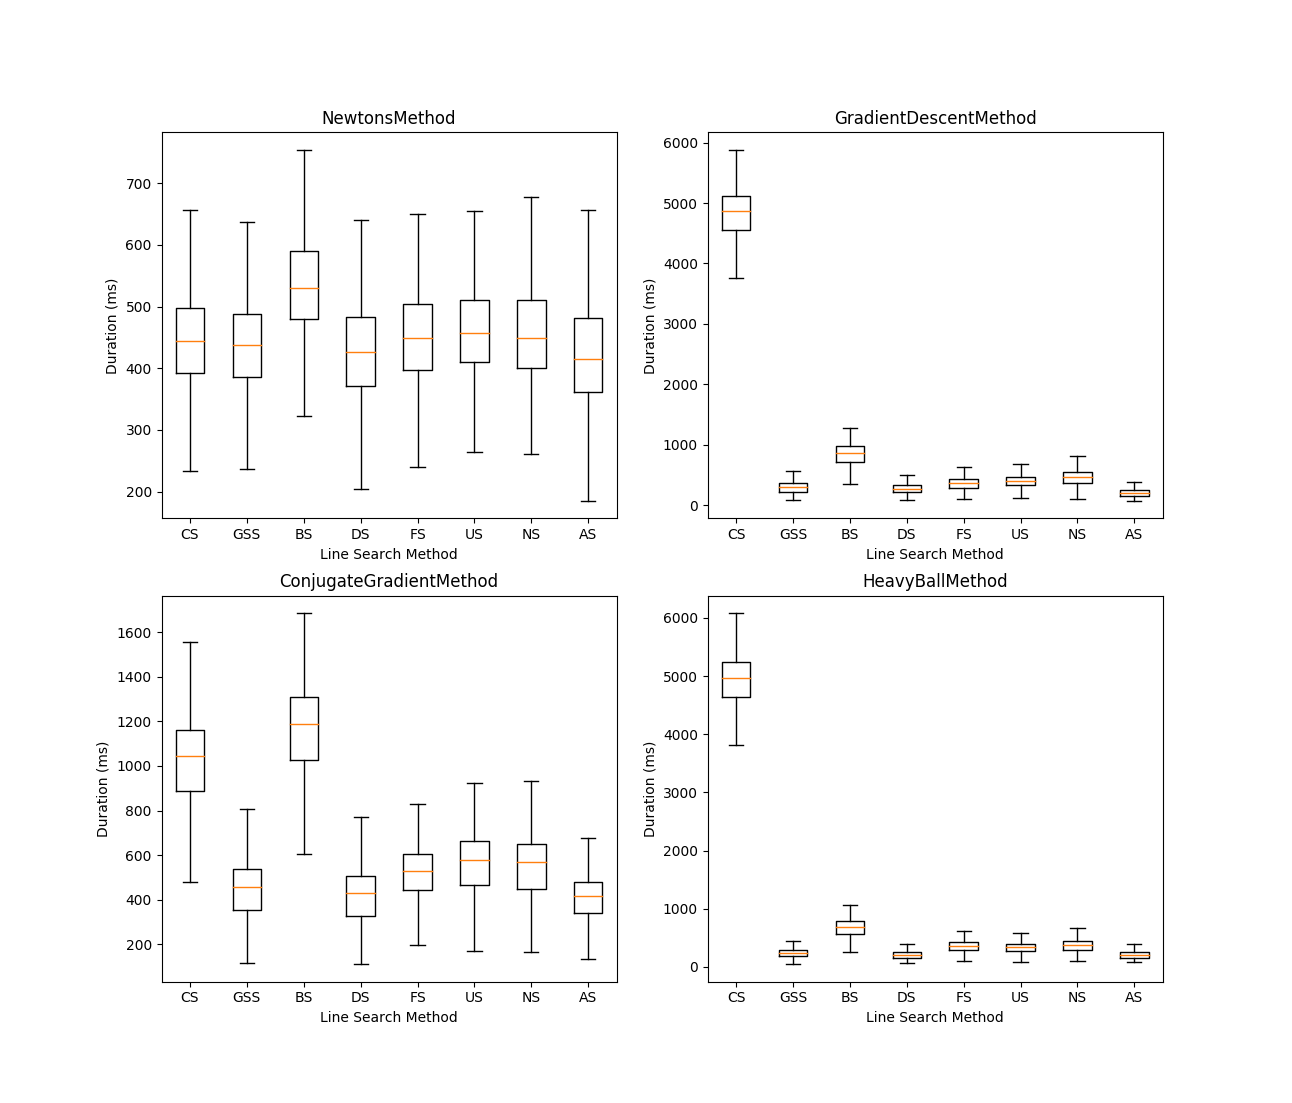
\includegraphics[width=1.0\textwidth]{images/boxplot_mss.png}
	\caption{Box plot of solution times per line search and main method for MatrixSquareSum target function.}
	\label{fig:boxplot_mss}
\end{figure}


\begin{figure}[H]
	\centering
	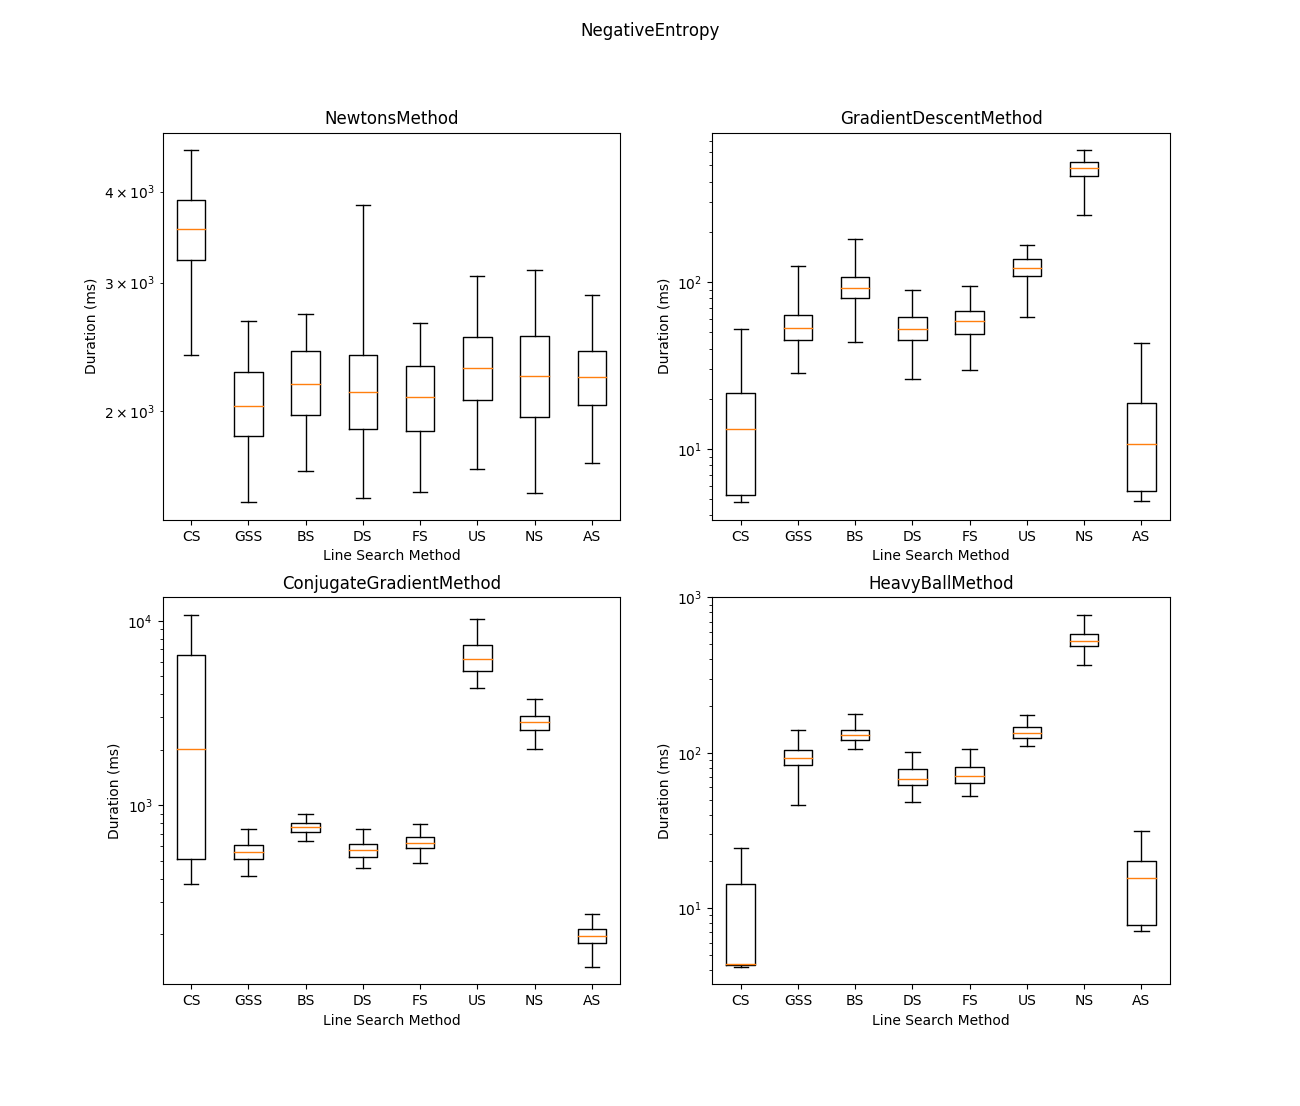
\includegraphics[width=1.0\textwidth]{images/boxplot_ne.png}
	\caption{Box plot of solution times per line search and main method for NegativeEntropy target function.}
	\label{fig:boxplot_ne}
\end{figure}

\todoinline{Explain the box plot method. Apparently the box contains 50\% of the dataset and the lines rest or smthing like that?}
%https://matplotlib.org/3.1.1/gallery/statistics/boxplot_demo.html
%https://towardsdatascience.com/understanding-boxplots-5e2df7bcbd51



% From the tables \ref{tab:scores_rank_target_function} to \ref{tab:scores_duration_main_method} we can clearly see that there are indeed some differences between the performances of the methods. Analysing the per target function ranking table (table \ref{tab:scores_rank_target_function}), which takes into account both the success rate and average duration, we can see that Armijo's Search has the best total results in both target function scenarios. Not that far behind is Dichotomous Search and also Golden Section Search with really solid performances. The worst performer was Bisection Search followed by Uniform and Newton's Searches. While Uniform Search was expected to score bad due to its straight forward nature, it is a bit suprising to see both methods using derivatives score so low on the comparison. This is however a fact that may well be heavily effected by the selection of target functions alone.

% While the table \ref{tab:scores_rank_main_method} tells us mostly the same story as the previous one, there are still some interesting new aspects to note from here. First and foremost it seems that while Armijo's Search is still superior in overall performance, it severely lacks behind in performance in case of Newton's Method. Looking back at the raw results in tables \ref{tab:performance_results_MSS_NM} and \ref{tab:performance_results_NE_NM}, we can see that this is indeed the case but only for combination of Newton's Method with Matrix Square Sum target function. Overall the results seem to have taken a surprising turn in case of Newton's Method since the overall worst performers Uniform Search, Newton's Search and even Constant Search have scored the highest ranks for this setup. And while Golden Section Search seems to have scored pretty average score, a closer look into the table \ref{tab:performance_results_MSS_NM} reveals that the differences in performance were minimal, which can be clearly seen if we..

\subsubsection{Constant Search}

Since Constant Search simply provides us constant step sizes it should be used as a baseline for other line search methods. It will not take any time to compute the step size so the main stress remains on the main method and how well can it find the solution with never changing step size.

% The results for Constant Search look surprisingly good at first: from the overall ranking table (table \ref{tab:scores_rank_target_function}) we can see that while constant step size did not score too well on Matrix Square Sum, it seems like the second strongest choice for Negative Entropy target function. However, taking a closer look at the actual average durations in tables \ref{tab:scores_duration_target_function} and \ref{tab:scores_duration_main_method} we notice that the situation is a bit different. The Constant Search has scored the bottom or close to bottom score for all target functions and for each main method. Investigating this further, we can see from tables \ref{tab:performance_results_MSS_NM} to \ref{tab:performance_results_NE_HBM} that the Constant Search scored really well on Gradient Descent and Heavy Ball Methods for Negative Entropy function explaining the above average ranking. Since this was mainly an issue caused by the choice of ranking algorithm, it is safe to say that Constant Search performed largely as expected as can be seen from the high average durations from the tables \ref{tab:scores_duration_target_function} and \ref{tab:scores_duration_main_method}. However, as the data tells us, there exists scenarios in which with a good choice of main method and target function, Constant Search may prove itself really effective, but these scenarios should most likely be tested beforehand to avoid otherwise not just poor completion time but below average success rate.


\section{Conclusion and Future Research}


To make the results completely comprehensive we should consider all existing functions as possible target functions. However as this is practically impossible, one substantial way to improve the coverage would be increasing the number of target functions: other similar research has used up to 80 different problems to calculate the performance for \cite{monotone_line_search_performance},

Another major factor in increasing the reliability of the results are the starting points. In this research we limited the area of where the points were generated to $[-10, 10]$ or $]0, 10]$ depending on the domain of the target function. In a perfect world we could test the algorithms for every single starting point. Even though that is practically impossible, a wider range of points could be utilized. Anyways the selection of starting point is very target function related and should always be considered per function. In addition the number of starting points tested could be raised within the computing power available.


% %
% % LÄHDELUETTELO
% %  BibTeX-tiedoston kokoaminen onnistuu näppärästi esim. 
% %  Firefoxin Zotero-lisäosalla http://www.zotero.org/
% %  joka osaa poimia viitteet suoraan Google Scholarista.
% %
\newpage
% \bibliographystyle{plainnat}
\bibliographystyle{abbrvnat}
%\bibliographystyle{plain} % valitse tämä jos et käytä natbib-pakettia

% Ladataan library.bib
\bibliography{library}


% %
% % LIITTEET
% %
% \newpage
% \appendix
% \section{Ensimmäinen liite}

\newpage
\section{Attachments}
% TODO: enable

\subsection{Constant Search}
\begin{figure}[H]
\captionof{figure}{Best parameter permutations for different main methods using ConstantSearch for optimizing the MatrixSquareSum function with 10 sample points.}
\label{fig:param_comp_MatrixSquareSum_ConstantSearch}
\begin{subfigure}[ht]{.5\textwidth}
\rowcolors{2}{white}{gray!5}
\begin{tabular}{|c|c|c|}
\hline
\rowcolor{gray!25}
\multicolumn{3}{|c|}{NewtonsMethod} \\
\hline
\rowcolor{gray!25}
$(\lambda)$ & $s$ (\%) & $t$ (ms) \\
\hline
(1.0,) & 100.0 & 436.3 \\
(0.9,) & 100.0 & 4072.7 \\
(1.1,) & 100.0 & 4389.6 \\
(1.5,) & 100.0 & 11768.2 \\
(0.5,) & 100.0 & 13857.0 \\
\hline
\end{tabular}
\caption{Top 5 permutations with NewtonsMethod}
\label{subfig:param_comp_MatrixSquareSum_NewtonsMethod_ConstantSearch}
\end{subfigure}
\hfill
\begin{subfigure}[ht]{.5\textwidth}
\rowcolors{2}{white}{gray!5}
\begin{tabular}{|c|c|c|}
\hline
\rowcolor{gray!25}
\multicolumn{3}{|c|}{GradientDescentMethod} \\
\hline
\rowcolor{gray!25}
$(\lambda)$ & $s$ (\%) & $t$ (ms) \\
\hline
(0.0001,) & 100.0 & 8299.9 \\
(0.5,) & 0.0 & 162.8 \\
(0.9,) & 0.0 & 169.7 \\
(0.1,) & 0.0 & 187.9 \\
(0.25,) & 0.0 & 193.4 \\
\hline
\end{tabular}
\caption{Top 5 permutations with GradientDescentMethod}
\label{subfig:param_comp_MatrixSquareSum_GradientDescentMethod_ConstantSearch}
\end{subfigure}
\hfill
\begin{subfigure}[ht]{.5\textwidth}
\rowcolors{2}{white}{gray!5}
\begin{tabular}{|c|c|c|}
\hline
\rowcolor{gray!25}
\multicolumn{3}{|c|}{ConjugateGradientMethod} \\
\hline
\rowcolor{gray!25}
$(\lambda)$ & $s$ (\%) & $t$ (ms) \\
\hline
(0.0001,) & 100.0 & 1054.7 \\
(0.1,) & 0.0 & 192.4 \\
(0.5,) & 0.0 & 270.2 \\
(0.25,) & 0.0 & 280.1 \\
(0.9,) & 0.0 & 298.0 \\
\hline
\end{tabular}
\caption{Top 5 permutations with ConjugateGradientMethod}
\label{subfig:param_comp_MatrixSquareSum_ConjugateGradientMethod_ConstantSearch}
\end{subfigure}
\hfill
\begin{subfigure}[ht]{.5\textwidth}
\rowcolors{2}{white}{gray!5}
\begin{tabular}{|c|c|c|}
\hline
\rowcolor{gray!25}
\multicolumn{3}{|c|}{HeavyBallMethod} \\
\hline
\rowcolor{gray!25}
$(\lambda,\beta_{HBM})$ & $s$ (\%) & $t$ (ms) \\
\hline
(0.0001, 0.1) & 100.0 & 6437.8 \\
(0.0001, 0.5) & 100.0 & 6580.6 \\
(0.0001, 10.0) & 100.0 & 6714.6 \\
(0.0001, 5.0) & 100.0 & 6784.6 \\
(0.0001, 1.0) & 100.0 & 6838.7 \\
\hline
\end{tabular}
\caption{Top 5 permutations with HeavyBallMethod}
\label{subfig:param_comp_MatrixSquareSum_HeavyBallMethod_ConstantSearch}
\end{subfigure}
\end{figure}

\begin{figure}[H]
\captionof{figure}{Best parameter permutations for different main methods using ConstantSearch for optimizing the NegativeEntropy function with 10 sample points.}
\label{fig:param_comp_NegativeEntropy_ConstantSearch}
\begin{subfigure}[ht]{.5\textwidth}
\rowcolors{2}{white}{gray!5}
\begin{tabular}{|c|c|c|}
\hline
\rowcolor{gray!25}
\multicolumn{3}{|c|}{NewtonsMethod} \\
\hline
\rowcolor{gray!25}
$(\lambda)$ & $s$ (\%) & $t$ (ms) \\
\hline
(0.9,) & 100.0 & 3379.7 \\
(0.5,) & 100.0 & 7239.4 \\
(0.25,) & 100.0 & 17055.7 \\
(0.1,) & 100.0 & 46295.4 \\
\hline
\end{tabular}
\caption{Top 5 permutations with NewtonsMethod}
\label{subfig:param_comp_NegativeEntropy_NewtonsMethod_ConstantSearch}
\end{subfigure}
\hfill
\begin{subfigure}[ht]{.5\textwidth}
\rowcolors{2}{white}{gray!5}
\begin{tabular}{|c|c|c|}
\hline
\rowcolor{gray!25}
\multicolumn{3}{|c|}{GradientDescentMethod} \\
\hline
\rowcolor{gray!25}
$(\lambda)$ & $s$ (\%) & $t$ (ms) \\
\hline
(0.5,) & 100.0 & 17.8 \\
(0.25,) & 100.0 & 57.5 \\
(0.1,) & 100.0 & 226.9 \\
\hline
\end{tabular}
\caption{Top 5 permutations with GradientDescentMethod}
\label{subfig:param_comp_NegativeEntropy_GradientDescentMethod_ConstantSearch}
\end{subfigure}
\hfill
\begin{subfigure}[ht]{.5\textwidth}
\rowcolors{2}{white}{gray!5}
\begin{tabular}{|c|c|c|}
\hline
\rowcolor{gray!25}
\multicolumn{3}{|c|}{ConjugateGradientMethod} \\
\hline
\rowcolor{gray!25}
$(\lambda)$ & $s$ (\%) & $t$ (ms) \\
\hline
(0.1,) & 100.0 & 2361.4 \\
(0.0001,) & 100.0 & 4281.1 \\
(0.15,) & 100.0 & 4969.4 \\
(0.2,) & 100.0 & 6062.7 \\
\hline
\end{tabular}
\caption{Top 5 permutations with ConjugateGradientMethod}
\label{subfig:param_comp_NegativeEntropy_ConjugateGradientMethod_ConstantSearch}
\end{subfigure}
\hfill
\begin{subfigure}[ht]{.5\textwidth}
\rowcolors{2}{white}{gray!5}
\begin{tabular}{|c|c|c|}
\hline
\rowcolor{gray!25}
\multicolumn{3}{|c|}{HeavyBallMethod} \\
\hline
\rowcolor{gray!25}
$(\lambda,\beta_{HBM})$ & $s$ (\%) & $t$ (ms) \\
\hline
(0.5, 0.1) & 100.0 & 9.1 \\
(0.5, 0.5) & 100.0 & 14.7 \\
(0.25, 0.1) & 100.0 & 15.3 \\
(0.25, 0.5) & 100.0 & 15.8 \\
(0.25, 1.0) & 100.0 & 18.2 \\
\hline
\end{tabular}
\caption{Top 5 permutations with HeavyBallMethod}
\label{subfig:param_comp_NegativeEntropy_HeavyBallMethod_ConstantSearch}
\end{subfigure}
\end{figure}

\subsection{Golden Section Search}
\begin{center}
\rowcolors{2}{white}{gray!5}
\captionof{table}{Parameters tested for GoldenSectionSearch}
\label{tab:params_GoldenSectionSearch}
\begin{tabular}{|c|c|c|}
\hline
\rowcolor{gray!25}
Parameter & MatrixSquareSum & NegativeEntropy \\
\hline
$a$ & -10, -5 & -10, -5 \\
$b$ & 10, 5 & 10, 5 \\
$l$ & 0.0001, 1e-07 & 0.0001, 1e-07 \\
\hline
\end{tabular}
\end{center}

\begin{figure}[H]
\captionof{figure}{Best parameter permutations for different main methods using GoldenSectionSearch for optimizing the MatrixSquareSum function with 10 sample points.}
\label{fig:param_comp_MatrixSquareSum_GoldenSectionSearch}
\begin{subfigure}[ht]{.5\textwidth}
\rowcolors{2}{white}{gray!5}
\begin{tabular}{|c|c|c|}
\hline
\rowcolor{gray!25}
\multicolumn{3}{|c|}{NewtonsMethod} \\
\hline
\rowcolor{gray!25}
$(a,b,l)$ & $s$ (\%) & $t$ (ms) \\
\hline
(-10, 5, 1e-07) & 100.0 & 515.6 \\
(-10, 10, 1e-07) & 100.0 & 868.6 \\
(-10, 10, 0.0001) & 100.0 & 887.5 \\
(-5, 5, 1e-07) & 100.0 & 891.0 \\
(-5, 10, 0.0001) & 100.0 & 914.0 \\
\hline
\end{tabular}
\caption{Top 5 permutations with NewtonsMethod}
\label{subfig:param_comp_MatrixSquareSum_NewtonsMethod_GoldenSectionSearch}
\end{subfigure}
\hfill
\begin{subfigure}[ht]{.5\textwidth}
\rowcolors{2}{white}{gray!5}
\begin{tabular}{|c|c|c|}
\hline
\rowcolor{gray!25}
\multicolumn{3}{|c|}{GradientDescentMethod} \\
\hline
\rowcolor{gray!25}
$(a,b,l)$ & $s$ (\%) & $t$ (ms) \\
\hline
(-10, 5, 0.0001) & 100.0 & 279.4 \\
(-5, 10, 0.0001) & 100.0 & 318.0 \\
(-5, 5, 0.0001) & 100.0 & 344.3 \\
(-10, 5, 1e-07) & 100.0 & 371.1 \\
(-10, 10, 0.0001) & 100.0 & 379.6 \\
\hline
\end{tabular}
\caption{Top 5 permutations with GradientDescentMethod}
\label{subfig:param_comp_MatrixSquareSum_GradientDescentMethod_GoldenSectionSearch}
\end{subfigure}
\hfill
\begin{subfigure}[ht]{.5\textwidth}
\rowcolors{2}{white}{gray!5}
\begin{tabular}{|c|c|c|}
\hline
\rowcolor{gray!25}
\multicolumn{3}{|c|}{ConjugateGradientMethod} \\
\hline
\rowcolor{gray!25}
$(a,b,l)$ & $s$ (\%) & $t$ (ms) \\
\hline
(-5, 10, 0.0001) & 100.0 & 436.7 \\
(-10, 10, 0.0001) & 100.0 & 467.8 \\
(-5, 5, 0.0001) & 100.0 & 489.2 \\
(-10, 5, 0.0001) & 100.0 & 529.8 \\
(-10, 10, 1e-07) & 100.0 & 533.9 \\
\hline
\end{tabular}
\caption{Top 5 permutations with ConjugateGradientMethod}
\label{subfig:param_comp_MatrixSquareSum_ConjugateGradientMethod_GoldenSectionSearch}
\end{subfigure}
\hfill
\begin{subfigure}[ht]{.5\textwidth}
\rowcolors{2}{white}{gray!5}
\begin{tabular}{|c|c|c|}
\hline
\rowcolor{gray!25}
\multicolumn{3}{|c|}{HeavyBallMethod} \\
\hline
\rowcolor{gray!25}
$(a,b,l,\beta_{HBM})$ & $s$ (\%) & $t$ (ms) \\
\hline
(-5, 10, 0.0001, 10.0) & 100.0 & 230.6 \\
(-10, 5, 0.0001, 10.0) & 100.0 & 236.7 \\
(-10, 10, 0.0001, 10.0) & 100.0 & 243.6 \\
(-5, 10, 0.0001, 5.0) & 100.0 & 244.8 \\
(-5, 5, 0.0001, 10.0) & 100.0 & 252.1 \\
\hline
\end{tabular}
\caption{Top 5 permutations with HeavyBallMethod}
\label{subfig:param_comp_MatrixSquareSum_HeavyBallMethod_GoldenSectionSearch}
\end{subfigure}
\end{figure}

\begin{figure}[H]
\captionof{figure}{Best parameter permutations for different main methods using GoldenSectionSearch for optimizing the NegativeEntropy function with 10 sample points.}
\label{fig:param_comp_NegativeEntropy_GoldenSectionSearch}
\begin{subfigure}[ht]{.5\textwidth}
\rowcolors{2}{white}{gray!5}
\begin{tabular}{|c|c|c|}
\hline
\rowcolor{gray!25}
\multicolumn{3}{|c|}{NewtonsMethod} \\
\hline
\rowcolor{gray!25}
$(a,b,l)$ & $s$ (\%) & $t$ (ms) \\
\hline
(-5, 5, 1e-07) & 100.0 & 1758.0 \\
(-10, 5, 0.0001) & 100.0 & 1905.6 \\
(-10, 10, 0.0001) & 100.0 & 1946.7 \\
(-10, 10, 1e-07) & 100.0 & 1947.3 \\
(-5, 5, 0.0001) & 100.0 & 1968.5 \\
\hline
\end{tabular}
\caption{Top 5 permutations with NewtonsMethod}
\label{subfig:param_comp_NegativeEntropy_NewtonsMethod_GoldenSectionSearch}
\end{subfigure}
\hfill
\begin{subfigure}[ht]{.5\textwidth}
\rowcolors{2}{white}{gray!5}
\begin{tabular}{|c|c|c|}
\hline
\rowcolor{gray!25}
\multicolumn{3}{|c|}{GradientDescentMethod} \\
\hline
\rowcolor{gray!25}
$(a,b,l)$ & $s$ (\%) & $t$ (ms) \\
\hline
(-5, 5, 0.0001) & 100.0 & 57.1 \\
(-5, 5, 1e-07) & 100.0 & 68.4 \\
(-5, 10, 0.0001) & 100.0 & 85.4 \\
(-5, 10, 1e-07) & 100.0 & 85.8 \\
(-10, 5, 1e-07) & 100.0 & 109.9 \\
\hline
\end{tabular}
\caption{Top 5 permutations with GradientDescentMethod}
\label{subfig:param_comp_NegativeEntropy_GradientDescentMethod_GoldenSectionSearch}
\end{subfigure}
\hfill
\begin{subfigure}[ht]{.5\textwidth}
\rowcolors{2}{white}{gray!5}
\begin{tabular}{|c|c|c|}
\hline
\rowcolor{gray!25}
\multicolumn{3}{|c|}{ConjugateGradientMethod} \\
\hline
\rowcolor{gray!25}
$(a,b,l)$ & $s$ (\%) & $t$ (ms) \\
\hline
(-5, 5, 0.0001) & 100.0 & 591.3 \\
(-10, 5, 0.0001) & 100.0 & 644.1 \\
(-5, 5, 1e-07) & 100.0 & 644.4 \\
(-5, 10, 0.0001) & 100.0 & 648.5 \\
(-10, 5, 1e-07) & 100.0 & 672.1 \\
\hline
\end{tabular}
\caption{Top 5 permutations with ConjugateGradientMethod}
\label{subfig:param_comp_NegativeEntropy_ConjugateGradientMethod_GoldenSectionSearch}
\end{subfigure}
\hfill
\begin{subfigure}[ht]{.5\textwidth}
\rowcolors{2}{white}{gray!5}
\begin{tabular}{|c|c|c|}
\hline
\rowcolor{gray!25}
\multicolumn{3}{|c|}{HeavyBallMethod} \\
\hline
\rowcolor{gray!25}
$(a,b,l,\beta_{HBM})$ & $s$ (\%) & $t$ (ms) \\
\hline
(-5, 5, 0.0001, 0.1) & 100.0 & 72.3 \\
(-10, 5, 0.0001, 0.1) & 100.0 & 75.0 \\
(-5, 10, 0.0001, 0.1) & 100.0 & 75.2 \\
(-5, 5, 1e-07, 0.1) & 100.0 & 79.7 \\
(-5, 10, 1e-07, 0.1) & 100.0 & 80.4 \\
\hline
\end{tabular}
\caption{Top 5 permutations with HeavyBallMethod}
\label{subfig:param_comp_NegativeEntropy_HeavyBallMethod_GoldenSectionSearch}
\end{subfigure}
\end{figure}

\subsection{Bisection Search}
\begin{figure}[H]
\captionof{figure}{Best parameter permutations for different main methods using BisectionSearch for optimizing the MatrixSquareSum function with 10 sample points.}
\label{fig:param_comp_MatrixSquareSum_BisectionSearch}
\begin{subfigure}[ht]{.5\textwidth}
\rowcolors{2}{white}{gray!5}
\begin{tabular}{|c|c|c|}
\hline
\rowcolor{gray!25}
\multicolumn{3}{|c|}{NewtonsMethod} \\
\hline
\rowcolor{gray!25}
$(a,b,l)$ & $s$ (\%) & $t$ (ms) \\
\hline
(-10, 5, 1e-07) & 100.0 & 555.4 \\
(-5, 10, 1e-07) & 100.0 & 597.9 \\
(-5, 5, 1e-07) & 100.0 & 962.4 \\
(-10, 5, 0.0001) & 100.0 & 1025.9 \\
(-10, 10, 0.0001) & 100.0 & 1049.4 \\
\hline
\end{tabular}
\caption{Top 5 permutations with NewtonsMethod}
\label{subfig:param_comp_MatrixSquareSum_NewtonsMethod_BisectionSearch}
\end{subfigure}
\hfill
\begin{subfigure}[ht]{.5\textwidth}
\rowcolors{2}{white}{gray!5}
\begin{tabular}{|c|c|c|}
\hline
\rowcolor{gray!25}
\multicolumn{3}{|c|}{GradientDescentMethod} \\
\hline
\rowcolor{gray!25}
$(a,b,l)$ & $s$ (\%) & $t$ (ms) \\
\hline
(-10, 5, 0.0001) & 100.0 & 836.1 \\
(-5, 5, 0.0001) & 100.0 & 911.2 \\
(-10, 10, 0.0001) & 100.0 & 921.0 \\
(-5, 10, 0.0001) & 100.0 & 956.1 \\
(-5, 5, 1e-07) & 100.0 & 1094.3 \\
\hline
\end{tabular}
\caption{Top 5 permutations with GradientDescentMethod}
\label{subfig:param_comp_MatrixSquareSum_GradientDescentMethod_BisectionSearch}
\end{subfigure}
\hfill
\begin{subfigure}[ht]{.5\textwidth}
\rowcolors{2}{white}{gray!5}
\begin{tabular}{|c|c|c|}
\hline
\rowcolor{gray!25}
\multicolumn{3}{|c|}{ConjugateGradientMethod} \\
\hline
\rowcolor{gray!25}
$(a,b,l)$ & $s$ (\%) & $t$ (ms) \\
\hline
(-10, 10, 0.0001) & 100.0 & 1152.1 \\
(-5, 5, 0.0001) & 100.0 & 1153.7 \\
(-10, 5, 0.0001) & 100.0 & 1157.4 \\
(-5, 10, 0.0001) & 100.0 & 1175.7 \\
(-5, 10, 1e-07) & 100.0 & 1575.7 \\
\hline
\end{tabular}
\caption{Top 5 permutations with ConjugateGradientMethod}
\label{subfig:param_comp_MatrixSquareSum_ConjugateGradientMethod_BisectionSearch}
\end{subfigure}
\hfill
\begin{subfigure}[ht]{.5\textwidth}
\rowcolors{2}{white}{gray!5}
\begin{tabular}{|c|c|c|}
\hline
\rowcolor{gray!25}
\multicolumn{3}{|c|}{HeavyBallMethod} \\
\hline
\rowcolor{gray!25}
$(a,b,l,\beta_{HBM})$ & $s$ (\%) & $t$ (ms) \\
\hline
(-10, 10, 0.0001, 10.0) & 100.0 & 581.2 \\
(-5, 10, 0.0001, 5.0) & 100.0 & 627.6 \\
(-5, 10, 0.0001, 10.0) & 100.0 & 676.6 \\
(-5, 5, 0.0001, 10.0) & 100.0 & 706.7 \\
(-5, 5, 0.0001, 5.0) & 100.0 & 714.3 \\
\hline
\end{tabular}
\caption{Top 5 permutations with HeavyBallMethod}
\label{subfig:param_comp_MatrixSquareSum_HeavyBallMethod_BisectionSearch}
\end{subfigure}
\end{figure}

\begin{figure}[H]
\captionof{figure}{Best parameter permutations for different main methods using BisectionSearch for optimizing the NegativeEntropy function with 10 sample points.}
\label{fig:param_comp_NegativeEntropy_BisectionSearch}
\begin{subfigure}[ht]{.5\textwidth}
\rowcolors{2}{white}{gray!5}
\begin{tabular}{|c|c|c|}
\hline
\rowcolor{gray!25}
\multicolumn{3}{|c|}{NewtonsMethod} \\
\hline
\rowcolor{gray!25}
$(a,b,l)$ & $s$ (\%) & $t$ (ms) \\
\hline
(-10, 10, 0.0001) & 100.0 & 1753.5 \\
(-10, 5, 0.0001) & 100.0 & 2006.3 \\
(-5, 5, 1e-07) & 100.0 & 2044.7 \\
(-5, 10, 0.0001) & 100.0 & 2075.4 \\
(-5, 5, 0.0001) & 100.0 & 2162.0 \\
\hline
\end{tabular}
\caption{Top 5 permutations with NewtonsMethod}
\label{subfig:param_comp_NegativeEntropy_NewtonsMethod_BisectionSearch}
\end{subfigure}
\hfill
\begin{subfigure}[ht]{.5\textwidth}
\rowcolors{2}{white}{gray!5}
\begin{tabular}{|c|c|c|}
\hline
\rowcolor{gray!25}
\multicolumn{3}{|c|}{GradientDescentMethod} \\
\hline
\rowcolor{gray!25}
$(a,b,l)$ & $s$ (\%) & $t$ (ms) \\
\hline
(-5, 5, 0.0001) & 100.0 & 105.5 \\
(-10, 5, 0.0001) & 100.0 & 114.6 \\
(-5, 10, 0.0001) & 100.0 & 115.6 \\
(-10, 5, 1e-07) & 100.0 & 128.9 \\
(-5, 5, 1e-07) & 100.0 & 136.3 \\
\hline
\end{tabular}
\caption{Top 5 permutations with GradientDescentMethod}
\label{subfig:param_comp_NegativeEntropy_GradientDescentMethod_BisectionSearch}
\end{subfigure}
\hfill
\begin{subfigure}[ht]{.5\textwidth}
\rowcolors{2}{white}{gray!5}
\begin{tabular}{|c|c|c|}
\hline
\rowcolor{gray!25}
\multicolumn{3}{|c|}{ConjugateGradientMethod} \\
\hline
\rowcolor{gray!25}
$(a,b,l)$ & $s$ (\%) & $t$ (ms) \\
\hline
(-5, 5, 0.0001) & 100.0 & 883.4 \\
(-10, 10, 0.0001) & 100.0 & 891.5 \\
(-10, 5, 0.0001) & 100.0 & 893.8 \\
(-5, 10, 0.0001) & 100.0 & 916.2 \\
(-10, 5, 1e-07) & 100.0 & 1092.6 \\
\hline
\end{tabular}
\caption{Top 5 permutations with ConjugateGradientMethod}
\label{subfig:param_comp_NegativeEntropy_ConjugateGradientMethod_BisectionSearch}
\end{subfigure}
\hfill
\begin{subfigure}[ht]{.5\textwidth}
\rowcolors{2}{white}{gray!5}
\begin{tabular}{|c|c|c|}
\hline
\rowcolor{gray!25}
\multicolumn{3}{|c|}{HeavyBallMethod} \\
\hline
\rowcolor{gray!25}
$(a,b,l,\beta_{HBM})$ & $s$ (\%) & $t$ (ms) \\
\hline
(-10, 10, 0.0001, 0.1) & 100.0 & 138.9 \\
(-5, 5, 0.0001, 0.1) & 100.0 & 142.4 \\
(-10, 5, 0.0001, 0.1) & 100.0 & 153.4 \\
(-5, 10, 0.0001, 0.1) & 100.0 & 154.3 \\
(-5, 5, 0.0001, 0.5) & 100.0 & 182.9 \\
\hline
\end{tabular}
\caption{Top 5 permutations with HeavyBallMethod}
\label{subfig:param_comp_NegativeEntropy_HeavyBallMethod_BisectionSearch}
\end{subfigure}
\end{figure}

\subsection{Dichotomous Search}
\begin{figure}[H]
\captionof{figure}{Best parameter permutations for different main methods using DichotomousSearch for optimizing the MatrixSquareSum function with 10 sample points.}
\label{fig:param_comp_MatrixSquareSum_DichotomousSearch}
\makebox[\linewidth][c]{
\begin{subfigure}[ht]{.6\textwidth}
\centering
\rowcolors{2}{white}{gray!5}
\begin{tabular}{|c|c|c|}
\hline
\rowcolor{gray!25}
\multicolumn{3}{|c|}{NewtonsMethod} \\
\hline
\rowcolor{gray!25}
$(a,b,\epsilon,l)$ & $s$ (\%) & $t$ (ms) \\
\hline
(-5, 10, 1e-10, 1e-09) & 100.0 & 388.3 \\
(-10, 10, 1e-10, 1e-09) & 100.0 & 436.4 \\
(-5, 5, 1e-10, 1e-09) & 100.0 & 439.6 \\
(-10, 5, 1e-10, 1e-09) & 100.0 & 455.0 \\
(-5, 10, 1e-07, 1e-05) & 100.0 & 840.8 \\
\hline
\end{tabular}
\caption{Top 5 permutations with NewtonsMethod}
\label{subfig:param_comp_MatrixSquareSum_NewtonsMethod_DichotomousSearch}
\end{subfigure}
\hfill
\begin{subfigure}[ht]{.6\textwidth}
\centering
\rowcolors{2}{white}{gray!5}
\begin{tabular}{|c|c|c|}
\hline
\rowcolor{gray!25}
\multicolumn{3}{|c|}{GradientDescentMethod} \\
\hline
\rowcolor{gray!25}
$(a,b,\epsilon,l)$ & $s$ (\%) & $t$ (ms) \\
\hline
(-10, 5, 1e-07, 1e-05) & 100.0 & 234.8 \\
(-10, 5, 1e-08, 0.0001) & 100.0 & 241.2 \\
(-5, 5, 1e-07, 0.0001) & 100.0 & 252.5 \\
(-5, 10, 1e-08, 0.0001) & 100.0 & 252.9 \\
(-10, 5, 1e-08, 1e-05) & 100.0 & 260.4 \\
\hline
\end{tabular}
\caption{Top 5 permutations with GradientDescentMethod}
\label{subfig:param_comp_MatrixSquareSum_GradientDescentMethod_DichotomousSearch}
\end{subfigure}
}
\makebox[\linewidth][c]{
\begin{subfigure}[ht]{.6\textwidth}
\centering
\rowcolors{2}{white}{gray!5}
\begin{tabular}{|c|c|c|}
\hline
\rowcolor{gray!25}
\multicolumn{3}{|c|}{ConjugateGradientMethod} \\
\hline
\rowcolor{gray!25}
$(a,b,\epsilon,l)$ & $s$ (\%) & $t$ (ms) \\
\hline
(-5, 10, 1e-07, 1e-05) & 100.0 & 354.2 \\
(-5, 10, 1e-07, 0.0001) & 100.0 & 382.0 \\
(-5, 5, 1e-07, 0.0001) & 100.0 & 397.3 \\
(-10, 10, 1e-08, 1e-05) & 100.0 & 406.2 \\
(-10, 5, 1e-08, 0.0001) & 100.0 & 406.7 \\
\hline
\end{tabular}
\caption{Top 5 permutations with ConjugateGradientMethod}
\label{subfig:param_comp_MatrixSquareSum_ConjugateGradientMethod_DichotomousSearch}
\end{subfigure}
\hfill
\begin{subfigure}[ht]{.6\textwidth}
\centering
\rowcolors{2}{white}{gray!5}
\begin{tabular}{|c|c|c|}
\hline
\rowcolor{gray!25}
\multicolumn{3}{|c|}{HeavyBallMethod} \\
\hline
\rowcolor{gray!25}
$(a,b,\epsilon,l,\beta_{HBM})$ & $s$ (\%) & $t$ (ms) \\
\hline
(-5, 5, 1e-07, 0.0001, 10.0) & 100.0 & 173.6 \\
(-10, 10, 1e-07, 0.0001, 10.0) & 100.0 & 185.4 \\
(-5, 10, 1e-08, 0.0001, 10.0) & 100.0 & 193.9 \\
(-10, 5, 1e-08, 1e-05, 5.0) & 100.0 & 202.6 \\
(-5, 5, 1e-07, 1e-05, 10.0) & 100.0 & 205.2 \\
\hline
\end{tabular}
\caption{Top 5 permutations with HeavyBallMethod}
\label{subfig:param_comp_MatrixSquareSum_HeavyBallMethod_DichotomousSearch}
\end{subfigure}
}
\end{figure}

\begin{figure}[H]
\captionof{figure}{Best parameter permutations for different main methods using DichotomousSearch for optimizing the NegativeEntropy function with 10 sample points.}
\label{fig:param_comp_NegativeEntropy_DichotomousSearch}
\makebox[\linewidth][c]{
\begin{subfigure}[ht]{.6\textwidth}
\centering
\rowcolors{2}{white}{gray!5}
\begin{tabular}{|c|c|c|}
\hline
\rowcolor{gray!25}
\multicolumn{3}{|c|}{NewtonsMethod} \\
\hline
\rowcolor{gray!25}
$(a,b,\epsilon,l)$ & $s$ (\%) & $t$ (ms) \\
\hline
(-10, 10, 1e-07, 1e-05) & 100.0 & 1756.0 \\
(-10, 5, 1e-06, 1e-05) & 100.0 & 1846.8 \\
(-10, 10, 1e-06, 0.0001) & 100.0 & 1882.9 \\
(-10, 5, 1e-06, 0.0001) & 100.0 & 1893.5 \\
(-10, 10, 1e-06, 1e-05) & 100.0 & 1923.0 \\
\hline
\end{tabular}
\caption{Top 5 permutations with NewtonsMethod}
\label{subfig:param_comp_NegativeEntropy_NewtonsMethod_DichotomousSearch}
\end{subfigure}
\hfill
\begin{subfigure}[ht]{.6\textwidth}
\centering
\rowcolors{2}{white}{gray!5}
\begin{tabular}{|c|c|c|}
\hline
\rowcolor{gray!25}
\multicolumn{3}{|c|}{GradientDescentMethod} \\
\hline
\rowcolor{gray!25}
$(a,b,\epsilon,l)$ & $s$ (\%) & $t$ (ms) \\
\hline
(-5, 5, 1e-07, 0.0001) & 100.0 & 54.3 \\
(-5, 10, 1e-06, 0.0001) & 100.0 & 61.7 \\
(-5, 10, 1e-06, 1e-05) & 100.0 & 63.8 \\
(-5, 5, 1e-07, 1e-05) & 100.0 & 64.6 \\
(-5, 10, 1e-07, 0.0001) & 100.0 & 65.4 \\
\hline
\end{tabular}
\caption{Top 5 permutations with GradientDescentMethod}
\label{subfig:param_comp_NegativeEntropy_GradientDescentMethod_DichotomousSearch}
\end{subfigure}
}
\makebox[\linewidth][c]{
\begin{subfigure}[ht]{.6\textwidth}
\centering
\rowcolors{2}{white}{gray!5}
\begin{tabular}{|c|c|c|}
\hline
\rowcolor{gray!25}
\multicolumn{3}{|c|}{ConjugateGradientMethod} \\
\hline
\rowcolor{gray!25}
$(a,b,\epsilon,l)$ & $s$ (\%) & $t$ (ms) \\
\hline
(-5, 5, 1e-06, 0.0001) & 100.0 & 640.6 \\
(-10, 5, 1e-06, 0.0001) & 100.0 & 642.7 \\
(-5, 5, 1e-07, 0.0001) & 100.0 & 645.3 \\
(-5, 10, 1e-07, 0.0001) & 100.0 & 657.0 \\
(-5, 5, 1e-06, 1e-05) & 100.0 & 680.9 \\
\hline
\end{tabular}
\caption{Top 5 permutations with ConjugateGradientMethod}
\label{subfig:param_comp_NegativeEntropy_ConjugateGradientMethod_DichotomousSearch}
\end{subfigure}
\hfill
\begin{subfigure}[ht]{.6\textwidth}
\centering
\rowcolors{2}{white}{gray!5}
\begin{tabular}{|c|c|c|}
\hline
\rowcolor{gray!25}
\multicolumn{3}{|c|}{HeavyBallMethod} \\
\hline
\rowcolor{gray!25}
$(a,b,\epsilon,l,\beta_{HBM})$ & $s$ (\%) & $t$ (ms) \\
\hline
(-5, 5, 1e-06, 1e-05, 0.1) & 100.0 & 70.4 \\
(-5, 5, 1e-06, 0.0001, 0.1) & 100.0 & 70.8 \\
(-10, 5, 1e-07, 0.0001, 0.1) & 100.0 & 73.3 \\
(-5, 10, 1e-06, 0.0001, 0.1) & 100.0 & 74.0 \\
(-5, 5, 1e-07, 0.0001, 0.1) & 100.0 & 74.0 \\
\hline
\end{tabular}
\caption{Top 5 permutations with HeavyBallMethod}
\label{subfig:param_comp_NegativeEntropy_HeavyBallMethod_DichotomousSearch}
\end{subfigure}
}
\end{figure}

\subsection{Fibonacci Search}
\begin{figure}[H]
\captionof{figure}{Best parameter permutations for different main methods using FibonacciSearch for optimizing the MatrixSquareSum function with 10 sample points.}
\label{fig:param_comp_MatrixSquareSum_FibonacciSearch}
\makebox[\linewidth][c]{
\begin{subfigure}[ht]{.6\textwidth}
\centering
\rowcolors{2}{white}{gray!5}
\begin{tabular}{|c|c|c|}
\hline
\rowcolor{gray!25}
\multicolumn{3}{|c|}{NewtonsMethod} \\
\hline
\rowcolor{gray!25}
$(a,b,\epsilon,l)$ & $s$ (\%) & $t$ (ms) \\
\hline
(-5, 5, 1e-10, 1e-10) & 100.0 & 443.2 \\
(-5, 5, 1e-12, 1e-10) & 100.0 & 452.3 \\
(-5, 5, 1e-08, 1e-10) & 100.0 & 459.6 \\
(-10, 5, 1e-10, 1e-10) & 100.0 & 460.9 \\
(-10, 5, 1e-12, 1e-10) & 100.0 & 469.7 \\
\hline
\end{tabular}
\caption{Top 5 permutations with NewtonsMethod}
\label{subfig:param_comp_MatrixSquareSum_NewtonsMethod_FibonacciSearch}
\end{subfigure}
\hfill
\begin{subfigure}[ht]{.6\textwidth}
\centering
\rowcolors{2}{white}{gray!5}
\begin{tabular}{|c|c|c|}
\hline
\rowcolor{gray!25}
\multicolumn{3}{|c|}{GradientDescentMethod} \\
\hline
\rowcolor{gray!25}
$(a,b,\epsilon,l)$ & $s$ (\%) & $t$ (ms) \\
\hline
(-5, 10, 1e-12, 1e-06) & 100.0 & 355.6 \\
(-5, 10, 1e-10, 1e-06) & 100.0 & 356.0 \\
(-5, 5, 1e-12, 1e-06) & 100.0 & 366.8 \\
(-10, 10, 1e-12, 1e-06) & 100.0 & 369.2 \\
(-10, 5, 1e-12, 1e-06) & 100.0 & 369.4 \\
\hline
\end{tabular}
\caption{Top 5 permutations with GradientDescentMethod}
\label{subfig:param_comp_MatrixSquareSum_GradientDescentMethod_FibonacciSearch}
\end{subfigure}
}
\makebox[\linewidth][c]{
\begin{subfigure}[ht]{.6\textwidth}
\centering
\rowcolors{2}{white}{gray!5}
\begin{tabular}{|c|c|c|}
\hline
\rowcolor{gray!25}
\multicolumn{3}{|c|}{ConjugateGradientMethod} \\
\hline
\rowcolor{gray!25}
$(a,b,\epsilon,l)$ & $s$ (\%) & $t$ (ms) \\
\hline
(-5, 10, 1e-10, 1e-06) & 100.0 & 473.8 \\
(-10, 10, 1e-10, 1e-06) & 100.0 & 485.0 \\
(-5, 10, 1e-12, 1e-06) & 100.0 & 490.3 \\
(-10, 5, 1e-08, 1e-06) & 100.0 & 508.6 \\
(-10, 10, 1e-12, 1e-06) & 100.0 & 516.0 \\
\hline
\end{tabular}
\caption{Top 5 permutations with ConjugateGradientMethod}
\label{subfig:param_comp_MatrixSquareSum_ConjugateGradientMethod_FibonacciSearch}
\end{subfigure}
\hfill
\begin{subfigure}[ht]{.6\textwidth}
\centering
\rowcolors{2}{white}{gray!5}
\begin{tabular}{|c|c|c|}
\hline
\rowcolor{gray!25}
\multicolumn{3}{|c|}{HeavyBallMethod} \\
\hline
\rowcolor{gray!25}
$(a,b,\epsilon,l,\beta_{HBM})$ & $s$ (\%) & $t$ (ms) \\
\hline
(-10, 5, 1e-12, 1e-06, 10.0) & 100.0 & 251.4 \\
(-5, 5, 1e-12, 1e-06, 10.0) & 100.0 & 268.5 \\
(-5, 5, 1e-08, 1e-06, 10.0) & 100.0 & 273.0 \\
(-10, 10, 1e-12, 1e-06, 10.0) & 100.0 & 273.5 \\
(-5, 5, 1e-10, 1e-06, 10.0) & 100.0 & 273.5 \\
\hline
\end{tabular}
\caption{Top 5 permutations with HeavyBallMethod}
\label{subfig:param_comp_MatrixSquareSum_HeavyBallMethod_FibonacciSearch}
\end{subfigure}
}
\end{figure}

\begin{figure}[H]
\captionof{figure}{Best parameter permutations for different main methods using FibonacciSearch for optimizing the NegativeEntropy function with 10 sample points.}
\label{fig:param_comp_NegativeEntropy_FibonacciSearch}
\makebox[\linewidth][c]{
\begin{subfigure}[ht]{.6\textwidth}
\centering
\rowcolors{2}{white}{gray!5}
\begin{tabular}{|c|c|c|}
\hline
\rowcolor{gray!25}
\multicolumn{3}{|c|}{NewtonsMethod} \\
\hline
\rowcolor{gray!25}
$(a,b,\epsilon,l)$ & $s$ (\%) & $t$ (ms) \\
\hline
(-5, 5, 1e-12, 1e-12) & 100.0 & 1834.0 \\
(-10, 5, 1e-08, 1e-06) & 100.0 & 1908.9 \\
(-10, 10, 1e-12, 1e-06) & 100.0 & 1946.8 \\
(-5, 10, 1e-10, 1e-06) & 100.0 & 1957.9 \\
(-10, 10, 1e-10, 1e-06) & 100.0 & 1967.3 \\
\hline
\end{tabular}
\caption{Top 5 permutations with NewtonsMethod}
\label{subfig:param_comp_NegativeEntropy_NewtonsMethod_FibonacciSearch}
\end{subfigure}
\hfill
\begin{subfigure}[ht]{.6\textwidth}
\centering
\rowcolors{2}{white}{gray!5}
\begin{tabular}{|c|c|c|}
\hline
\rowcolor{gray!25}
\multicolumn{3}{|c|}{GradientDescentMethod} \\
\hline
\rowcolor{gray!25}
$(a,b,\epsilon,l)$ & $s$ (\%) & $t$ (ms) \\
\hline
(-5, 5, 1e-12, 1e-06) & 100.0 & 74.5 \\
(-5, 10, 1e-08, 1e-06) & 100.0 & 75.8 \\
(-5, 5, 1e-10, 1e-06) & 100.0 & 78.0 \\
(-5, 5, 1e-08, 1e-06) & 100.0 & 78.3 \\
(-10, 5, 1e-12, 1e-12) & 100.0 & 78.6 \\
\hline
\end{tabular}
\caption{Top 5 permutations with GradientDescentMethod}
\label{subfig:param_comp_NegativeEntropy_GradientDescentMethod_FibonacciSearch}
\end{subfigure}
}
\makebox[\linewidth][c]{
\begin{subfigure}[ht]{.6\textwidth}
\centering
\rowcolors{2}{white}{gray!5}
\begin{tabular}{|c|c|c|}
\hline
\rowcolor{gray!25}
\multicolumn{3}{|c|}{ConjugateGradientMethod} \\
\hline
\rowcolor{gray!25}
$(a,b,\epsilon,l)$ & $s$ (\%) & $t$ (ms) \\
\hline
(-5, 5, 1e-08, 1e-06) & 100.0 & 682.8 \\
(-5, 5, 1e-12, 1e-06) & 100.0 & 683.5 \\
(-5, 5, 1e-10, 1e-06) & 100.0 & 701.5 \\
(-10, 5, 1e-10, 1e-06) & 100.0 & 728.0 \\
(-5, 10, 1e-08, 1e-06) & 100.0 & 729.5 \\
\hline
\end{tabular}
\caption{Top 5 permutations with ConjugateGradientMethod}
\label{subfig:param_comp_NegativeEntropy_ConjugateGradientMethod_FibonacciSearch}
\end{subfigure}
\hfill
\begin{subfigure}[ht]{.6\textwidth}
\centering
\rowcolors{2}{white}{gray!5}
\begin{tabular}{|c|c|c|}
\hline
\rowcolor{gray!25}
\multicolumn{3}{|c|}{HeavyBallMethod} \\
\hline
\rowcolor{gray!25}
$(a,b,\epsilon,l,\beta_{HBM})$ & $s$ (\%) & $t$ (ms) \\
\hline
(-5, 5, 1e-12, 1e-06, 0.1) & 100.0 & 76.4 \\
(-5, 5, 1e-10, 1e-06, 0.1) & 100.0 & 82.2 \\
(-10, 5, 1e-08, 1e-06, 0.1) & 100.0 & 85.1 \\
(-5, 10, 1e-10, 1e-06, 0.1) & 100.0 & 86.9 \\
(-5, 5, 1e-08, 1e-06, 0.1) & 100.0 & 87.6 \\
\hline
\end{tabular}
\caption{Top 5 permutations with HeavyBallMethod}
\label{subfig:param_comp_NegativeEntropy_HeavyBallMethod_FibonacciSearch}
\end{subfigure}
}
\end{figure}

\subsection{Uniform Search}
\begin{figure}[H]
\captionof{figure}{Best parameter permutations for different main methods using UniformSearch for optimizing the MatrixSquareSum function with 10 sample points.}
\label{fig:param_comp_MatrixSquareSum_UniformSearch}
\makebox[\linewidth][c]{
\begin{subfigure}[ht]{.6\textwidth}
\centering
\rowcolors{2}{white}{gray!5}
\begin{tabular}{|c|c|c|}
\hline
\rowcolor{gray!25}
\multicolumn{3}{|c|}{NewtonsMethod} \\
\hline
\rowcolor{gray!25}
$(a,b,n,m,l)$ & $s$ (\%) & $t$ (ms) \\
\hline
(-10, 5, 5, 1.5, 1e-06) & 100.0 & 424.0 \\
(-5, 5, 10, 1.5, 1e-06) & 100.0 & 424.5 \\
(-5, 5, 10, 1, 1e-08) & 100.0 & 449.1 \\
(-10, 10, 5, 1.5, 1e-08) & 100.0 & 459.5 \\
(-5, 10, 5, 1, 1e-06) & 100.0 & 463.1 \\
\hline
\end{tabular}
\caption{Top 5 permutations with NewtonsMethod}
\label{subfig:param_comp_MatrixSquareSum_NewtonsMethod_UniformSearch}
\end{subfigure}
\hfill
\begin{subfigure}[ht]{.6\textwidth}
\centering
\rowcolors{2}{white}{gray!5}
\begin{tabular}{|c|c|c|}
\hline
\rowcolor{gray!25}
\multicolumn{3}{|c|}{GradientDescentMethod} \\
\hline
\rowcolor{gray!25}
$(a,b,n,m,l)$ & $s$ (\%) & $t$ (ms) \\
\hline
(-10, 5, 5, 1, 1e-06) & 100.0 & 231.0 \\
(-5, 5, 5, 1, 1e-06) & 100.0 & 254.0 \\
(-5, 10, 5, 1, 1e-06) & 100.0 & 287.5 \\
(-5, 10, 10, 1, 1e-06) & 100.0 & 289.1 \\
(-5, 5, 5, 1, 1e-08) & 100.0 & 381.7 \\
\hline
\end{tabular}
\caption{Top 5 permutations with GradientDescentMethod}
\label{subfig:param_comp_MatrixSquareSum_GradientDescentMethod_UniformSearch}
\end{subfigure}
}
\makebox[\linewidth][c]{
\begin{subfigure}[ht]{.6\textwidth}
\centering
\rowcolors{2}{white}{gray!5}
\begin{tabular}{|c|c|c|}
\hline
\rowcolor{gray!25}
\multicolumn{3}{|c|}{ConjugateGradientMethod} \\
\hline
\rowcolor{gray!25}
$(a,b,n,m,l)$ & $s$ (\%) & $t$ (ms) \\
\hline
(-5, 10, 5, 1, 1e-06) & 100.0 & 328.1 \\
(-10, 10, 5, 1, 1e-06) & 100.0 & 364.8 \\
(-5, 5, 5, 1, 1e-06) & 100.0 & 371.5 \\
(-10, 5, 5, 1, 1e-06) & 100.0 & 378.8 \\
(-5, 5, 10, 1, 1e-06) & 100.0 & 529.3 \\
\hline
\end{tabular}
\caption{Top 5 permutations with ConjugateGradientMethod}
\label{subfig:param_comp_MatrixSquareSum_ConjugateGradientMethod_UniformSearch}
\end{subfigure}
\hfill
\begin{subfigure}[ht]{.6\textwidth}
\centering
\rowcolors{2}{white}{gray!5}
\begin{tabular}{|c|c|c|}
\hline
\rowcolor{gray!25}
\multicolumn{3}{|c|}{HeavyBallMethod} \\
\hline
\rowcolor{gray!25}
$(a,b,n,m,l,\beta_{HBM})$ & $s$ (\%) & $t$ (ms) \\
\hline
(-10, 10, 5, 1, 1e-06, 10.0) & 100.0 & 137.3 \\
(-5, 10, 5, 1, 1e-06, 10.0) & 100.0 & 155.6 \\
(-5, 5, 5, 1, 1e-06, 10.0) & 100.0 & 170.2 \\
(-10, 10, 5, 1, 1e-06, 5.0) & 100.0 & 185.4 \\
(-5, 5, 5, 1, 1e-06, 5.0) & 100.0 & 200.0 \\
\hline
\end{tabular}
\caption{Top 5 permutations with HeavyBallMethod}
\label{subfig:param_comp_MatrixSquareSum_HeavyBallMethod_UniformSearch}
\end{subfigure}
}
\end{figure}

\begin{figure}[H]
\captionof{figure}{Best parameter permutations for different main methods using UniformSearch for optimizing the NegativeEntropy function with 10 sample points.}
\label{fig:param_comp_NegativeEntropy_UniformSearch}
\makebox[\linewidth][c]{
\begin{subfigure}[ht]{.6\textwidth}
\centering
\rowcolors{2}{white}{gray!5}
\begin{tabular}{|c|c|c|}
\hline
\rowcolor{gray!25}
\multicolumn{3}{|c|}{NewtonsMethod} \\
\hline
\rowcolor{gray!25}
$(a,b,n,m,l)$ & $s$ (\%) & $t$ (ms) \\
\hline
(0, 5, 5, 1, 1e-05) & 100.0 & 1339.2 \\
(-5, 5, 5, 1, 1e-05) & 100.0 & 2047.3 \\
(-5, 10, 5, 1, 1e-05) & 100.0 & 2059.8 \\
(0, 5, 5, 1, 1e-06) & 100.0 & 2068.5 \\
(0, 5, 10, 1, 1e-06) & 100.0 & 2125.3 \\
\hline
\end{tabular}
\caption{Top 5 permutations with NewtonsMethod}
\label{subfig:param_comp_NegativeEntropy_NewtonsMethod_UniformSearch}
\end{subfigure}
\hfill
\begin{subfigure}[ht]{.6\textwidth}
\centering
\rowcolors{2}{white}{gray!5}
\begin{tabular}{|c|c|c|}
\hline
\rowcolor{gray!25}
\multicolumn{3}{|c|}{GradientDescentMethod} \\
\hline
\rowcolor{gray!25}
$(a,b,n,m,l)$ & $s$ (\%) & $t$ (ms) \\
\hline
(0, 5, 10, 1, 1e-05) & 100.0 & 139.2 \\
(0, 5, 10, 1.5, 1e-06) & 100.0 & 159.3 \\
(0, 5, 10, 1.5, 1e-05) & 100.0 & 160.6 \\
(0, 5, 10, 1, 1e-06) & 100.0 & 161.2 \\
(0, 5, 10, 2, 1e-06) & 100.0 & 169.0 \\
\hline
\end{tabular}
\caption{Top 5 permutations with GradientDescentMethod}
\label{subfig:param_comp_NegativeEntropy_GradientDescentMethod_UniformSearch}
\end{subfigure}
}
\makebox[\linewidth][c]{
\begin{subfigure}[ht]{.6\textwidth}
\centering
\rowcolors{2}{white}{gray!5}
\begin{tabular}{|c|c|c|}
\hline
\rowcolor{gray!25}
\multicolumn{3}{|c|}{ConjugateGradientMethod} \\
\hline
\rowcolor{gray!25}
$(a,b,n,m,l)$ & $s$ (\%) & $t$ (ms) \\
\hline
(0, 5, 10, 1, 1e-05) & 100.0 & 6718.5 \\
(0, 5, 5, 1, 1e-05) & 100.0 & 7035.3 \\
(-5, 5, 10, 1, 1e-05) & 100.0 & 7444.3 \\
(-5, 5, 5, 1, 1e-05) & 100.0 & 7807.4 \\
(0, 5, 5, 1.5, 1e-05) & 100.0 & 8299.8 \\
\hline
\end{tabular}
\caption{Top 5 permutations with ConjugateGradientMethod}
\label{subfig:param_comp_NegativeEntropy_ConjugateGradientMethod_UniformSearch}
\end{subfigure}
\hfill
\begin{subfigure}[ht]{.6\textwidth}
\centering
\rowcolors{2}{white}{gray!5}
\begin{tabular}{|c|c|c|}
\hline
\rowcolor{gray!25}
\multicolumn{3}{|c|}{HeavyBallMethod} \\
\hline
\rowcolor{gray!25}
$(a,b,n,m,l,\beta_{HBM})$ & $s$ (\%) & $t$ (ms) \\
\hline
(0, 5, 10, 1, 1e-05, 0.1) & 100.0 & 138.5 \\
(0, 5, 5, 1.5, 1e-05, 0.1) & 100.0 & 154.5 \\
(0, 5, 5, 1, 1e-05, 0.1) & 100.0 & 166.8 \\
(0, 5, 10, 1, 1e-06, 0.1) & 100.0 & 177.9 \\
(0, 5, 10, 1.5, 1e-05, 0.1) & 100.0 & 178.0 \\
\hline
\end{tabular}
\caption{Top 5 permutations with HeavyBallMethod}
\label{subfig:param_comp_NegativeEntropy_HeavyBallMethod_UniformSearch}
\end{subfigure}
}
\end{figure}

\subsection{Newton's Search}
\begin{center}
\rowcolors{2}{white}{gray!5}
\captionof{table}{Parameters tested for NewtonsSearch}
\label{tab:params_NewtonsSearch}
\begin{tabular}{|c|c|c|}
\hline
\rowcolor{gray!25}
Parameter & MatrixSquareSum & NegativeEntropy \\
\hline
$\lambda$ & 0.5, 1, 5, 10 & 0.1, 0.5, 1, 5 \\
$l$ & 1e-07, 1e-08 & 1e-07, 1e-08 \\
\hline
\end{tabular}
\end{center}

\begin{figure}[H]
\captionof{figure}{Best parameter permutations for different main methods using NewtonsSearch for optimizing the MatrixSquareSum function with 10 sample points.}
\label{fig:param_comp_MatrixSquareSum_NewtonsSearch}
\begin{subfigure}[ht]{.5\textwidth}
\rowcolors{2}{white}{gray!5}
\begin{tabular}{|c|c|c|}
\hline
\rowcolor{gray!25}
\multicolumn{3}{|c|}{NewtonsMethod} \\
\hline
\rowcolor{gray!25}
$(\lambda,l)$ & $s$ (\%) & $t$ (ms) \\
\hline
(1, 1e-07) & 100.0 & 411.3 \\
(10, 1e-08) & 100.0 & 435.8 \\
(1, 1e-08) & 100.0 & 445.1 \\
(5, 1e-08) & 100.0 & 447.9 \\
(5, 1e-07) & 100.0 & 449.2 \\
\hline
\end{tabular}
\caption{Top 5 permutations with NewtonsMethod}
\label{subfig:param_comp_MatrixSquareSum_NewtonsMethod_NewtonsSearch}
\end{subfigure}
\hfill
\begin{subfigure}[ht]{.5\textwidth}
\rowcolors{2}{white}{gray!5}
\begin{tabular}{|c|c|c|}
\hline
\rowcolor{gray!25}
\multicolumn{3}{|c|}{GradientDescentMethod} \\
\hline
\rowcolor{gray!25}
$(\lambda,l)$ & $s$ (\%) & $t$ (ms) \\
\hline
(1, 1e-08) & 100.0 & 412.0 \\
(5, 1e-07) & 100.0 & 415.6 \\
(10, 1e-07) & 100.0 & 430.2 \\
(5, 1e-08) & 100.0 & 460.3 \\
(10, 1e-08) & 100.0 & 470.8 \\
\hline
\end{tabular}
\caption{Top 5 permutations with GradientDescentMethod}
\label{subfig:param_comp_MatrixSquareSum_GradientDescentMethod_NewtonsSearch}
\end{subfigure}
\hfill
\begin{subfigure}[ht]{.5\textwidth}
\rowcolors{2}{white}{gray!5}
\begin{tabular}{|c|c|c|}
\hline
\rowcolor{gray!25}
\multicolumn{3}{|c|}{ConjugateGradientMethod} \\
\hline
\rowcolor{gray!25}
$(\lambda,l)$ & $s$ (\%) & $t$ (ms) \\
\hline
(1, 1e-07) & 100.0 & 502.4 \\
(0.5, 1e-07) & 100.0 & 537.2 \\
(10, 1e-08) & 100.0 & 554.9 \\
(5, 1e-07) & 100.0 & 569.9 \\
(1, 1e-08) & 100.0 & 592.0 \\
\hline
\end{tabular}
\caption{Top 5 permutations with ConjugateGradientMethod}
\label{subfig:param_comp_MatrixSquareSum_ConjugateGradientMethod_NewtonsSearch}
\end{subfigure}
\hfill
\begin{subfigure}[ht]{.5\textwidth}
\rowcolors{2}{white}{gray!5}
\begin{tabular}{|c|c|c|}
\hline
\rowcolor{gray!25}
\multicolumn{3}{|c|}{HeavyBallMethod} \\
\hline
\rowcolor{gray!25}
$(\lambda,l,\beta_{HBM})$ & $s$ (\%) & $t$ (ms) \\
\hline
(10, 1e-07, 10.0) & 100.0 & 338.8 \\
(5, 1e-07, 10.0) & 100.0 & 360.2 \\
(10, 1e-08, 5.0) & 100.0 & 361.5 \\
(0.5, 1e-07, 10.0) & 100.0 & 361.9 \\
(1, 1e-08, 10.0) & 100.0 & 382.9 \\
\hline
\end{tabular}
\caption{Top 5 permutations with HeavyBallMethod}
\label{subfig:param_comp_MatrixSquareSum_HeavyBallMethod_NewtonsSearch}
\end{subfigure}
\end{figure}

\begin{figure}[H]
\captionof{figure}{Best parameter permutations for different main methods using NewtonsSearch for optimizing the NegativeEntropy function with 10 sample points.}
\label{fig:param_comp_NegativeEntropy_NewtonsSearch}
\begin{subfigure}[ht]{.5\textwidth}
\rowcolors{2}{white}{gray!5}
\begin{tabular}{|c|c|c|}
\hline
\rowcolor{gray!25}
\multicolumn{3}{|c|}{NewtonsMethod} \\
\hline
\rowcolor{gray!25}
$(\lambda,l)$ & $s$ (\%) & $t$ (ms) \\
\hline
(0.5, 1e-08, 100) & 100.0 & 1659.8 \\
(1, 1e-08, 100) & 100.0 & 1662.6 \\
(1, 1e-07, 100) & 100.0 & 1671.8 \\
(5, 1e-07, 100) & 100.0 & 1707.0 \\
(0.5, 1e-07, 100) & 100.0 & 1723.9 \\
\hline
\end{tabular}
\caption{Top 5 permutations with NewtonsMethod}
\label{subfig:param_comp_NegativeEntropy_NewtonsMethod_NewtonsSearch}
\end{subfigure}
\hfill
\begin{subfigure}[ht]{.5\textwidth}
\rowcolors{2}{white}{gray!5}
\begin{tabular}{|c|c|c|}
\hline
\rowcolor{gray!25}
\multicolumn{3}{|c|}{GradientDescentMethod} \\
\hline
\rowcolor{gray!25}
$(\lambda,l)$ & $s$ (\%) & $t$ (ms) \\
\hline
(0.5, 1e-07, 100) & 100.0 & 476.2 \\
(0.5, 1e-08, 100) & 100.0 & 501.1 \\
(1, 1e-08, 100) & 100.0 & 501.8 \\
(0.1, 1e-08, 100) & 100.0 & 520.6 \\
(5, 1e-07, 100) & 100.0 & 521.0 \\
\hline
\end{tabular}
\caption{Top 5 permutations with GradientDescentMethod}
\label{subfig:param_comp_NegativeEntropy_GradientDescentMethod_NewtonsSearch}
\end{subfigure}
\hfill
\begin{subfigure}[ht]{.5\textwidth}
\rowcolors{2}{white}{gray!5}
\begin{tabular}{|c|c|c|}
\hline
\rowcolor{gray!25}
\multicolumn{3}{|c|}{ConjugateGradientMethod} \\
\hline
\rowcolor{gray!25}
$(\lambda,l)$ & $s$ (\%) & $t$ (ms) \\
\hline
(0.1, 1e-08, 100) & 100.0 & 2779.5 \\
(0.1, 1e-07, 100) & 100.0 & 2789.7 \\
(0.5, 1e-07, 100) & 100.0 & 2921.1 \\
(0.5, 1e-08, 100) & 100.0 & 2985.0 \\
(1, 1e-07, 100) & 100.0 & 3050.7 \\
\hline
\end{tabular}
\caption{Top 5 permutations with ConjugateGradientMethod}
\label{subfig:param_comp_NegativeEntropy_ConjugateGradientMethod_NewtonsSearch}
\end{subfigure}
\hfill
\begin{subfigure}[ht]{.5\textwidth}
\rowcolors{2}{white}{gray!5}
\begin{tabular}{|c|c|c|}
\hline
\rowcolor{gray!25}
\multicolumn{3}{|c|}{HeavyBallMethod} \\
\hline
\rowcolor{gray!25}
$(\lambda,l,\beta_{HBM})$ & $s$ (\%) & $t$ (ms) \\
\hline
(1, 1e-07, 100, 0.1) & 100.0 & 586.3 \\
(0.1, 1e-08, 100, 0.1) & 100.0 & 591.6 \\
(1, 1e-08, 100, 0.1) & 100.0 & 602.4 \\
(0.5, 1e-07, 100, 0.1) & 100.0 & 609.2 \\
(0.1, 1e-07, 100, 0.1) & 100.0 & 614.9 \\
\hline
\end{tabular}
\caption{Top 5 permutations with HeavyBallMethod}
\label{subfig:param_comp_NegativeEntropy_HeavyBallMethod_NewtonsSearch}
\end{subfigure}
\end{figure}

\subsection{Armijo's Search}
\begin{figure}[H]
\captionof{figure}{Best parameter permutations for different main methods using ArmijoSearch for optimizing the MatrixSquareSum function with 10 sample points.}
\label{fig:param_comp_MatrixSquareSum_ArmijoSearch}
\begin{subfigure}[ht]{.5\textwidth}
\rowcolors{2}{white}{gray!5}
\begin{tabular}{|c|c|c|}
\hline
\rowcolor{gray!25}
\multicolumn{3}{|c|}{NewtonsMethod} \\
\hline
\rowcolor{gray!25}
$(\lambda,\alpha,\beta)$ & $s$ (\%) & $t$ (ms) \\
\hline
(1, 0.1, 0.5) & 100.0 & 429.7 \\
(1, 0.25, 0.75) & 100.0 & 484.5 \\
(1, 0.25, 0.5) & 100.0 & 493.8 \\
(1, 0.25, 0.9) & 100.0 & 493.9 \\
(1, 0.1, 0.9) & 100.0 & 498.7 \\
\hline
\end{tabular}
\caption{Top 5 permutations with NewtonsMethod}
\label{subfig:param_comp_MatrixSquareSum_NewtonsMethod_ArmijoSearch}
\end{subfigure}
\hfill
\begin{subfigure}[ht]{.5\textwidth}
\rowcolors{2}{white}{gray!5}
\begin{tabular}{|c|c|c|}
\hline
\rowcolor{gray!25}
\multicolumn{3}{|c|}{GradientDescentMethod} \\
\hline
\rowcolor{gray!25}
$(\lambda,\alpha,\beta)$ & $s$ (\%) & $t$ (ms) \\
\hline
(1.1, 0.25, 0.5) & 100.0 & 143.0 \\
(1.1, 0.5, 0.5) & 100.0 & 211.3 \\
(1, 0.25, 0.5) & 100.0 & 215.6 \\
(0.9, 0.25, 0.5) & 100.0 & 216.4 \\
(0.9, 0.5, 0.5) & 100.0 & 236.4 \\
\hline
\end{tabular}
\caption{Top 5 permutations with GradientDescentMethod}
\label{subfig:param_comp_MatrixSquareSum_GradientDescentMethod_ArmijoSearch}
\end{subfigure}
\hfill
\begin{subfigure}[ht]{.5\textwidth}
\rowcolors{2}{white}{gray!5}
\begin{tabular}{|c|c|c|}
\hline
\rowcolor{gray!25}
\multicolumn{3}{|c|}{ConjugateGradientMethod} \\
\hline
\rowcolor{gray!25}
$(\lambda,\alpha,\beta)$ & $s$ (\%) & $t$ (ms) \\
\hline
(1.1, 0.25, 0.5) & 100.0 & 262.6 \\
(1, 0.25, 0.5) & 100.0 & 339.0 \\
(1.1, 0.1, 0.5) & 100.0 & 353.9 \\
(1, 0.25, 0.75) & 100.0 & 361.5 \\
(0.9, 0.25, 0.5) & 100.0 & 376.6 \\
\hline
\end{tabular}
\caption{Top 5 permutations with ConjugateGradientMethod}
\label{subfig:param_comp_MatrixSquareSum_ConjugateGradientMethod_ArmijoSearch}
\end{subfigure}
\hfill
\begin{subfigure}[ht]{.5\textwidth}
\rowcolors{2}{white}{gray!5}
\begin{tabular}{|c|c|c|}
\hline
\rowcolor{gray!25}
\multicolumn{3}{|c|}{HeavyBallMethod} \\
\hline
\rowcolor{gray!25}
$(\lambda,\alpha,\beta,\beta_{HBM})$ & $s$ (\%) & $t$ (ms) \\
\hline
(1.1, 0.25, 0.5, 0.1) & 100.0 & 142.5 \\
(0.9, 0.25, 0.5, 10.0) & 100.0 & 151.8 \\
(1, 0.25, 0.5, 10.0) & 100.0 & 165.7 \\
(1, 0.25, 0.5, 0.5) & 100.0 & 170.4 \\
(1.1, 0.5, 0.75, 10.0) & 100.0 & 173.8 \\
\hline
\end{tabular}
\caption{Top 5 permutations with HeavyBallMethod}
\label{subfig:param_comp_MatrixSquareSum_HeavyBallMethod_ArmijoSearch}
\end{subfigure}
\end{figure}

\begin{figure}[H]
\captionof{figure}{Best parameter permutations for different main methods using ArmijoSearch for optimizing the NegativeEntropy function with 10 sample points.}
\label{fig:param_comp_NegativeEntropy_ArmijoSearch}
\begin{subfigure}[ht]{.5\textwidth}
\rowcolors{2}{white}{gray!5}
\begin{tabular}{|c|c|c|}
\hline
\rowcolor{gray!25}
\multicolumn{3}{|c|}{NewtonsMethod} \\
\hline
\rowcolor{gray!25}
$(\lambda,\alpha,\beta)$ & $s$ (\%) & $t$ (ms) \\
\hline
(1.1, 0.5, 0.9) & 100.0 & 2094.1 \\
(1, 0.5, 0.75) & 100.0 & 2457.5 \\
(1, 0.5, 0.5) & 100.0 & 2659.1 \\
(1, 0.5, 0.9) & 100.0 & 2756.4 \\
(1.1, 0.25, 0.75) & 100.0 & 2854.2 \\
\hline
\end{tabular}
\caption{Top 5 permutations with NewtonsMethod}
\label{subfig:param_comp_NegativeEntropy_NewtonsMethod_ArmijoSearch}
\end{subfigure}
\hfill
\begin{subfigure}[ht]{.5\textwidth}
\rowcolors{2}{white}{gray!5}
\begin{tabular}{|c|c|c|}
\hline
\rowcolor{gray!25}
\multicolumn{3}{|c|}{GradientDescentMethod} \\
\hline
\rowcolor{gray!25}
$(\lambda,\alpha,\beta)$ & $s$ (\%) & $t$ (ms) \\
\hline
(1.1, 0.5, 0.75) & 100.0 & 11.2 \\
(1.1, 0.5, 0.9) & 100.0 & 12.6 \\
(0.9, 0.5, 0.9) & 100.0 & 12.7 \\
(1.1, 0.25, 0.75) & 100.0 & 13.9 \\
(1.1, 0.25, 0.5) & 100.0 & 15.4 \\
\hline
\end{tabular}
\caption{Top 5 permutations with GradientDescentMethod}
\label{subfig:param_comp_NegativeEntropy_GradientDescentMethod_ArmijoSearch}
\end{subfigure}
\hfill
\begin{subfigure}[ht]{.5\textwidth}
\rowcolors{2}{white}{gray!5}
\begin{tabular}{|c|c|c|}
\hline
\rowcolor{gray!25}
\multicolumn{3}{|c|}{ConjugateGradientMethod} \\
\hline
\rowcolor{gray!25}
$(\lambda,\alpha,\beta)$ & $s$ (\%) & $t$ (ms) \\
\hline
(0.9, 0.5, 0.5) & 100.0 & 221.7 \\
(1.1, 0.5, 0.5) & 100.0 & 242.8 \\
(0.9, 0.5, 0.75) & 100.0 & 252.2 \\
(1.1, 0.5, 0.75) & 100.0 & 255.0 \\
(1, 0.5, 0.5) & 100.0 & 262.5 \\
\hline
\end{tabular}
\caption{Top 5 permutations with ConjugateGradientMethod}
\label{subfig:param_comp_NegativeEntropy_ConjugateGradientMethod_ArmijoSearch}
\end{subfigure}
\hfill
\begin{subfigure}[ht]{.5\textwidth}
\rowcolors{2}{white}{gray!5}
\begin{tabular}{|c|c|c|}
\hline
\rowcolor{gray!25}
\multicolumn{3}{|c|}{HeavyBallMethod} \\
\hline
\rowcolor{gray!25}
$(\lambda,\alpha,\beta,\beta_{HBM})$ & $s$ (\%) & $t$ (ms) \\
\hline
(1, 0.5, 0.5, 0.1) & 100.0 & 11.4 \\
(1.1, 0.25, 0.5, 0.1) & 100.0 & 14.1 \\
(0.9, 0.5, 0.75, 0.1) & 100.0 & 14.5 \\
(0.9, 0.25, 0.5, 0.1) & 100.0 & 14.5 \\
(1, 0.5, 0.9, 0.1) & 100.0 & 15.8 \\
\hline
\end{tabular}
\caption{Top 5 permutations with HeavyBallMethod}
\label{subfig:param_comp_NegativeEntropy_HeavyBallMethod_ArmijoSearch}
\end{subfigure}
\end{figure}



\end{document}
